% =============================================================================
%  Technical documentation for the Rust VGA Kernel
%  Build with: latexmk -pdf main.tex   (or make)
% =============================================================================
\documentclass[11pt,a4paper,oneside]{report}

\usepackage[T1]{fontenc}
\usepackage[utf8]{inputenc}
\usepackage[english]{babel}
\usepackage{lmodern}
\usepackage{microtype}
\usepackage[a4paper,top=2.6cm,bottom=2.6cm,left=2.6cm,right=2.6cm]{geometry}

\usepackage{xcolor}
\usepackage{graphicx}
\usepackage{booktabs}
\usepackage{longtable}
\usepackage{array}
\usepackage{tabularx}
\usepackage{enumitem}
\usepackage{amssymb}
\usepackage{titlesec}
\usepackage{fancyhdr}
\usepackage{listings}
\usepackage[most]{tcolorbox}
\usepackage{tikz}
\usetikzlibrary{arrows.meta,positioning,shapes.geometric,fit,backgrounds,calc}
\usepackage{caption}
\usepackage{float}
\usepackage[hidelinks,unicode]{hyperref}

% -----------------------------------------------------------------------------
% Colors and style
% -----------------------------------------------------------------------------
\definecolor{rinuxblue}{HTML}{1F4E79}
\definecolor{rinuxlight}{HTML}{EAF1F8}
\definecolor{rinuxgray}{HTML}{4D4D4D}
\definecolor{codegreen}{HTML}{2E7D32}
\definecolor{codegray}{HTML}{6A737D}
\definecolor{codepurple}{HTML}{8E24AA}
\definecolor{codebackground}{HTML}{F6F8FA}

\titleformat{\chapter}[display]
  {\normalfont\bfseries\color{rinuxblue}}
  {\filright\Large Chapter \thechapter}
  {0.6ex}
  {\Huge}
\titlespacing*{\chapter}{0pt}{-10pt}{24pt}

\titleformat{\section}
  {\normalfont\Large\bfseries\color{rinuxblue}}{\thesection}{0.8em}{}
\titleformat{\subsection}
  {\normalfont\large\bfseries\color{rinuxgray}}{\thesubsection}{0.8em}{}

\pagestyle{fancy}
\fancyhf{}
\fancyhead[L]{\small\textcolor{rinuxgray}{Rust VGA Kernel --- Technical Documentation}}
\fancyhead[R]{\small\textcolor{rinuxgray}{\thepage}}
\renewcommand{\headrulewidth}{0.4pt}
\setlength{\headheight}{14pt}

\setlist[itemize]{topsep=2pt,itemsep=2pt,parsep=0pt}
\setlist[enumerate]{topsep=2pt,itemsep=2pt,parsep=0pt}

\captionsetup{font=small,labelfont=bf,width=0.95\linewidth}

% -----------------------------------------------------------------------------
% Listings (Rust)
% -----------------------------------------------------------------------------
\lstdefinelanguage{Rust}{
  keywords={as,break,const,continue,crate,else,enum,extern,false,fn,for,if,impl,in,let,loop,match,mod,move,mut,pub,ref,return,self,Self,static,struct,trait,true,type,unsafe,use,where,while,async,await,dyn,yield},
  keywordstyle=\color{rinuxblue}\bfseries,
  ndkeywords={u8,u16,u32,u64,usize,i32,bool,char,str,Option,Some,None,Result,Ok,Err,AtomicBool,UnsafeCell},
  ndkeywordstyle=\color{codepurple},
  sensitive=true,
  morecomment=[l]{//},
  morecomment=[s]{/*}{*/},
  morestring=[b]",
  morestring=[b]',
}

\lstset{
  language=Rust,
  backgroundcolor=\color{codebackground},
  basicstyle=\ttfamily\footnotesize,
  keywordstyle=\color{rinuxblue}\bfseries,
  commentstyle=\color{codegreen}\itshape,
  stringstyle=\color{codepurple},
  numbers=left,
  numberstyle=\tiny\color{codegray},
  numbersep=8pt,
  frame=single,
  rulecolor=\color{black!20},
  breaklines=true,
  breakatwhitespace=false,
  postbreak=\mbox{\textcolor{codegray}{$\hookrightarrow$}\space},
  showstringspaces=false,
  tabsize=4,
  captionpos=b,
  columns=fullflexible,
  keepspaces=true,
  upquote=true,
}

\lstdefinestyle{shell}{
  language={},
  basicstyle=\ttfamily\footnotesize,
  numbers=none,
  frame=single,
  backgroundcolor=\color{black!3},
}

% Highlight boxes
\newtcolorbox{nota}[1][]{
  enhanced, colback=rinuxlight, colframe=rinuxblue,
  boxrule=0.5pt, left=6pt, right=6pt, top=4pt, bottom=4pt,
  fonttitle=\bfseries, title=#1
}
\newtcolorbox{atencao}[1][]{
  enhanced, colback=orange!7, colframe=orange!70!black,
  boxrule=0.5pt, left=6pt, right=6pt, top=4pt, bottom=4pt,
  fonttitle=\bfseries, title=#1
}

\newcommand{\code}[1]{\texttt{#1}}
\newcommand{\termo}[1]{\textit{#1}}

% Metadata
\title{\vspace{-2cm}\textbf{Rust VGA Kernel}\\[0.4em]
       \Large Technical Documentation, Architecture and Comparison with Linux}
\author{Documentation generated from the source code}
\date{Version 1.0 --- November 3, 2026}

\begin{document}

\hypersetup{
  pdftitle={Rust VGA Kernel - Technical Documentation},
  pdfauthor={Rust VGA Kernel},
  pdfsubject={Minimal x86-64 kernel in Rust},
  pdfkeywords={Rust, kernel, x86-64, multiboot2, VGA, PS/2, Linux}
}

\maketitle

\begin{abstract}
This document describes the \textbf{Rust VGA Kernel} in full, an educational
kernel written in Rust with \code{no\_std} for standard BIOS/x86\_64 PCs.
The text covers the architecture, the boot chain, the memory model, the VGA
video, PS/2 keyboard and serial drivers, the built-in shell, the build and ISO
packaging process, the tests performed, and a quantitative and qualitative
analysis of how closely it resembles the Linux kernel.
The code implements the minimum path between the bootloader and a working
terminal, extended with an IDT, a timer, 4 KiB pages, \emph{demand paging}
and a demonstration of ring 3 code. It is not a port of Linux and does not
implement a scheduler, a heap, a filesystem or a complete set of system calls.
\end{abstract}

\tableofcontents
\listoffigures
\listoftables

\clearpage
\chapter{Introduction}
\label{cap:introducao}

\section{Motivation}

The Linux kernel is a complete operating system, with millions of lines of
code and decades of evolution. Studying how it works from the real code
requires traversing layers of abstraction, compilation configurations,
subsystems and code paths that are not essential to understanding the core of
the problem ``how does a computer go from boot to opening a terminal?''.

The \textbf{Rust VGA Kernel} was created as a didactic slice of that problem.
It reimplements, in Rust, the minimum path necessary to:

\begin{enumerate}
  \item be loaded by a standard bootloader (GRUB via Multiboot2);
  \item leave 32-bit mode and enter x86\_64 long mode;
  \item set up pages and a kernel stack;
  \item initialize an 80$\times$25 VGA text console;
  \item read keys from the PS/2 8042 controller and from the COM1 serial port;
  \item install an IDT, receive exceptions and the PIT timer;
  \item allocate 4 KiB frames and materialize pages on demand;
  \item execute code in ring 3 with user/kernel separation;
  \item offer a small shell with basic commands.
\end{enumerate}

The result is not a reduced Linux, nor a line-by-line port. It is an
independent kernel, with no external Rust dependencies, that reproduces
\emph{concepts} of the equivalent Linux subsystems at a comprehensible scale.

\section{Purpose of the document}

This documentation has four objectives:

\begin{itemize}
  \item \textbf{Explain the architecture} of the kernel: layers, boot flow,
        memory model, execution model and dependencies between modules.
  \item \textbf{Document the main functions} of each module, including
        contracts, preconditions, side effects and limitations.
        Appendix~\ref{ap:funcoes} contains the complete catalog of the
        project's 129 functions.
  \item \textbf{Record the build, execution and validation process}, so that
        another person can reproduce the environment and the tests.
  \item \textbf{Compare the project with the Linux kernel}, presenting
        correspondences of files and functions and a transparent estimate of
        the level of similarity.
\end{itemize}

\section{Scope}

\subsection*{What is included}

\begin{itemize}
  \item BIOS boot from CD/ISO using GRUB and the Multiboot2 protocol.
  \item Transition from 32 bits to long mode (x86\_64).
  \item GDT with ring 0/ring 3 segments, TSS and privilege stacks; static
        page tables at boot and the kernel's higher half.
  \item IDT with 256 gates, exceptions, remapped PIC and PIT timer on IRQ0.
  \item 4 KiB physical frame allocator and \emph{demand paging} for user and
        kernel regions.
  \item Ring 3 demos with U/S protection and a didactic
        \emph{syscall} \code{int \$0x80}.
  \item VGA console in text mode, with hardware cursor, scrolling and color
        attributes.
  \item PS/2 keyboard driver by \emph{polling}, with Shift, Enter, Tab and
        Backspace.
  \item UART 16550 driver on COM1, used for debugging and input.
  \item Shell without dynamic allocation with ten commands.
  \item \emph{Panic handler} that prints the failure and halts the CPU.
  \item Reproducible build with Cargo, \code{ld.lld}, \code{grub-mkrescue}
        and QEMU.
\end{itemize}

\subsection*{What is not included}

\begin{itemize}
  \item Heap, object allocator, \code{alloc} or dynamic collections.
  \item Complete processes, threads, scheduler, context switching, per-process
        address spaces or a broad set of system calls.
  \item Filesystem, networking, USB, ACPI, SMP or native UEFI support.
  \item Drivers for video modes other than the legacy VGA text mode.
  \item Security hardening such as SMEP, SMAP, NX, KASLR or validation of
        user pointers.
\end{itemize}

\section{Target audience}

The document is intended for:

\begin{itemize}
  \item students of operating systems and computer architecture;
  \item Rust developers interested in \code{no\_std} and bare metal;
  \item people who wish to understand the path between BIOS, bootloader and
        console before studying the Linux kernel in depth;
  \item reviewers who need to judge the degree of correspondence between this
        project and Linux.
\end{itemize}

\section{Conventions}

\begin{itemize}
  \item Code names appear in \code{monospaced font}.
  \item Hexadecimal addresses use the \code{0x} prefix.
  \item ``Higher half'' refers to addresses above
        \code{0xFFFF800000000000}, a convention used by Linux and by the
        \code{x86\_64-unknown-none} target.
  \item ``Original'' or ``Linux'' refers, unless stated otherwise, to the Linux
        7.3.1 tree used as the comparison reference.
  \item Address and section size values cited as ``observed'' were extracted
        from the reference compilation and may vary slightly between compiler
        versions.
\end{itemize}

\section{Project status}

The documented version is \code{0.1.0}, with the following characteristics:

\begin{table}[H]
\centering
\caption{Summary of the status of the documented version.}
\label{tab:estado}
\begin{tabularx}{\linewidth}{@{}lX@{}}
\toprule
\textbf{Item} & \textbf{Status} \\
\midrule
Compilation & \texttt{make} completes without errors; target \code{x86\_64-unknown-none}. \\
Image & \code{vga-kernel.iso} El Torito, bootable by BIOS. \\
Boot & Validated in QEMU with SeaBIOS and GRUB Multiboot2. \\
Console & VGA text 80$\times$25, cursor, scrolling and colors. \\
Input & PS/2 by polling and COM1 serial. \\
Interrupts & IDT with 256 gates, exceptions, remapped PIC and PIT at
~100 Hz. \\
Memory & 4 KiB frame allocator, 4 KiB tables and demand paging. \\
Protection & GDT/TSS, ring 3 and U/S bits for user and kernel. \\
Shell & \code{help}, \code{clear}, \code{echo}, \code{info}, \code{demand},
\code{usertest}, \code{userprot}, \code{mem}, \code{reboot}, \code{halt}. \\
Tests & Boot, commands, PS/2/serial input, timer, page faults and ring 3
verified. \\
Linux coverage & Small subset; low similarity (Chapter~\ref{cap:similaridade}). \\
\bottomrule
\end{tabularx}
\end{table}

\chapter{System overview}
\label{cap:visao}

\section{Executive summary}

The Rust VGA Kernel is an x86\_64 ELF executable loaded by GRUB. GRUB uses
the Multiboot2 protocol to transfer control to a small assembly-language
\emph{stub}, linked at 1 MiB. This stub builds page tables, enables PAE and
long mode and jumps to the Rust code, linked in the higher half at
\code{0xFFFFFFFF80000000}.

The Rust code initializes, in this order, the VGA renderer, the COM1 serial
port, the TTY layer with eight virtual consoles, the frame allocator, the GDT
with ring 3/TSS, the PS/2 keyboard and the IDT with PIC/PIT. It then enables
interrupts, prints a \emph{banner}, validates the Multiboot2 signature and
enters the shell, which displays the prompt \code{rinux>} on the active
console and processes commands read from the keyboard or from the serial
port.

The entire system fits in about 95 KiB of ELF and 3,223 lines of Rust
(2,477 effective lines of code, without comments and blank lines). There is no
dynamic heap allocation, scheduler or filesystem; there is an IDT, timer,
\emph{demand paging}, eight virtual consoles, four system calls and a
\code{getty}/login running in ring 3.

\section{Features}

\begin{table}[H]
\centering
\caption{Implemented features and their status.}
\label{tab:funcionalidades}
\begin{tabularx}{\linewidth}{@{}lXc@{}}
\toprule
\textbf{Area} & \textbf{Feature} & \textbf{Status} \\
\midrule
Boot & Valid Multiboot2 header & Complete \\
Boot & 32 $\rightarrow$ 64 bit transition & Complete \\
Memory & Static PML4/PDPT/PD, 1 GiB & Complete \\
Memory & Kernel higher half & Complete \\
Video & VGA text console 80$\times$25 & Complete \\
Video & Scrolling, cursor, tab, backspace & Complete \\
Video & Eight virtual consoles (\code{tty0}..\code{tty7}) & Complete \\
Video & Alt+F1..Alt+F8 and \code{tty} switching & Complete \\
Video & Graphics framebuffer / GOP & Absent \\
Keyboard & PS/2 8042, set 1, polling & Complete (subset) \\
Keyboard & Shift, Alt, Enter, Tab, Backspace & Complete \\
Keyboard & Alt+F1..Alt+F8 console selection & Complete \\
Keyboard & IRQ1, Caps Lock, AltGr, arrow keys & Absent \\
Serial & COM1 16550, 38400 8N1 & Complete (subset) \\
Serial & Input through the QEMU terminal & Complete \\
Shell & \code{help}, \code{clear}, \code{echo} & Complete \\
Shell & \code{info}, \code{tty}, \code{getty} & Complete \\
Shell & \code{reboot}, \code{halt} & Complete \\
System & Panic handler & Complete \\
System & IDT, exceptions and IRQ0 (timer) & Complete (subset) \\
System & GDT/TSS, ring 3 and U/S protection & Complete (demo) \\
System & Syscalls \code{exit/write/read/get\_tty} & Complete (subset) \\
User & \code{getty}/login in ring 3 & Complete (demo) \\
Memory & Frames, 4 KiB pages and demand paging & Complete (subset) \\
System & Heap, processes and scheduler & Absent \\
\bottomrule
\end{tabularx}
\end{table}

\section{Requirements}

\subsection{Hardware}

\begin{itemize}
  \item x86\_64-compatible PC with legacy BIOS or CSM enabled.
  \item PS/2 8042 keyboard controller (or equivalent emulation).
  \item VGA adapter in text mode, with a buffer at \code{0xB8000}.
  \item CD/DVD drive or equivalent device to boot the ISO.
  \item Enough memory to load the kernel and the ISO; 128 MiB is sufficient
        in QEMU.
\end{itemize}

\subsection{Development software}

\begin{itemize}
  \item Stable Rust with the \code{x86\_64-unknown-none} target installed.
  \item \code{rustup} (recommended; the Makefile prioritizes its toolchain).
  \item \code{ld.lld} (LLVM linker).
  \item \code{grub-mkrescue}, \code{xorriso}, \code{libisoburn} and
        \code{mtools}.
  \item QEMU (\code{qemu-system-x86\_64}) for execution and tests.
  \item For this documentation: a TeX Live distribution with
        \code{pdflatex} and \code{latexmk}.
\end{itemize}

\section{Directory structure}

\begin{lstlisting}[style=shell]
.
|-- Cargo.toml              metadados e perfis de compilacao
|-- Cargo.lock              lockfile (sem dependencias externas)
|-- rust-toolchain.toml     canal stable + alvo x86_64-unknown-none
|-- .cargo/config.toml      alvo padrao, linker e flags
|-- linker.ld               layout do ELF (stub baixo + kernel alto)
|-- Makefile                build do kernel, ISO e execucao no QEMU
|-- boot/grub/grub.cfg      menu Multiboot2 e console VGA
|-- src/
|   |-- main.rs             entrada Rust, macros e panic handler
|   |-- boot.rs             Multiboot2, GDT, paginacao e modo longo
|   |-- arch.rs             portas de I/O, interrupcoes, halt e reboot
|   |-- gdt.rs              GDT definitiva, TSS e pilhas de privilegio
|   |-- idt.rs              IDT, stubs, PIC, PIT e porta int 0x80
|   |-- paging.rs           frames, tabelas 4 KiB e demand paging
|   |-- user.rs             ring 3, demos e getty/login
|   |-- syscall.rs          exit/write/read/get_tty
|   |-- vga.rs              renderizador VGA 80x25
|   |-- tty.rs              consoles virtuais tty0..tty7
|   |-- keyboard.rs         teclado PS/2 (8042)
|   |-- serial.rs           UART 16550 / COM1
|   |-- shell.rs            prompt e comandos
|   `-- sync.rs             spinlock do console
|-- docs/                   esta documentacao (LaTeX e PDF)
|-- build/                  arvore temporaria da ISO (gerada)
|-- target/                 artefatos do Cargo (gerado)
|-- vga-kernel.iso          imagem inicializavel (gerada)
`-- README.md               guia rapido de uso
\end{lstlisting}

\section{Code metrics}

\begin{table}[H]
\centering
\caption{Metrics of the Rust modules (count by physical lines).}
\label{tab:metricas}
\begin{tabular}{@{}lrrl@{}}
\toprule
\textbf{Module} & \textbf{Lines} & \textbf{Functions} & \textbf{Responsibility} \\
\midrule
\code{boot.rs}     & 202 & 0 & Boot stub and page tables \\
\code{keyboard.rs} & 271 & 10 & PS/2 8042 driver \\
\code{vga.rs}      &  74 & 5 & VGA text renderer \\
\code{tty.rs}      & 448 & 31 & Virtual consoles and queues \\
\code{shell.rs}    & 245 & 9 & Command line and demos \\
\code{main.rs}     & 119 & 2 & Rust entry point, macros, panic \\
\code{serial.rs}   &  70 & 5 & UART 16550 / COM1 \\
\code{syscall.rs}  & 129 & 3 & exit/write/read/get\_tty \\
\code{arch.rs}     &  69 & 5 & I/O ports, \code{sti}, halt, reboot \\
\code{sync.rs}     &  56 & 5 & Spinlock \\
\code{gdt.rs}      & 159 & 7 & GDT, TSS and privilege stacks \\
\code{idt.rs}      & 504 & 14 & IDT, PIC, PIT, exceptions and IRQs \\
\code{paging.rs}   & 559 & 23 & Frames, tables and demand paging \\
\code{user.rs}     & 318 & 10 & Ring 3 entry, demos and getty \\
\midrule
\textbf{Total}     & \textbf{3,223} & \textbf{129} & 2,477 effective lines of code \\
\bottomrule
\end{tabular}
\end{table}

\begin{nota}[On the counting]
The count includes 351 comment lines and 395 blank lines. The number
of functions includes \code{impl} methods, \code{const} functions
and trait functions (\code{Deref}, \code{DerefMut}, \code{Drop} and
\code{fmt::Write}); it does not include \code{extern} declarations without a
body. \code{boot.rs} has no Rust functions because its logic is in
\code{global\_asm!}; the \emph{stub} is counted as an assembly block.
\end{nota}

\section{Summary of the execution flow}

\begin{enumerate}
  \item The BIOS selects the CD and executes El Torito.
  \item GRUB loads the ELF and reads the Multiboot2 header.
  \item GRUB enters 32-bit protected mode and jumps to \code{\_start}.
  \item The stub saves \code{eax} and \code{ebx}, builds the pages, loads the
        GDT and enables long mode.
  \item The stub jumps to \code{kernel\_main(magic, info)} in the higher half.
  \item Rust clears the VGA screen, configures the serial port, initializes
        the TTY layer with eight virtual consoles, initializes the frame
        allocator and the GDT/TSS, initializes the keyboard and installs the
        IDT with PIC/PIT.
  \item Rust enables interrupts and the shell displays \code{rinux>} on the
        active console, processing commands until \code{halt}, \code{reboot}
        or a physical reset.
\end{enumerate}

\chapter{Arquitetura}
\label{cap:arquitetura}

\section{Vis\~ao em camadas}

O kernel \'e organizado em cinco camadas conceituais. As camadas inferiores
dependem apenas de hardware e de \code{core}; as superiores usam as
inferiores. N\~ao h\'a \code{std}, alocador, \emph{runtime} de Rust nem
bibliotecas de terceiros.

\begin{figure}[H]
\centering
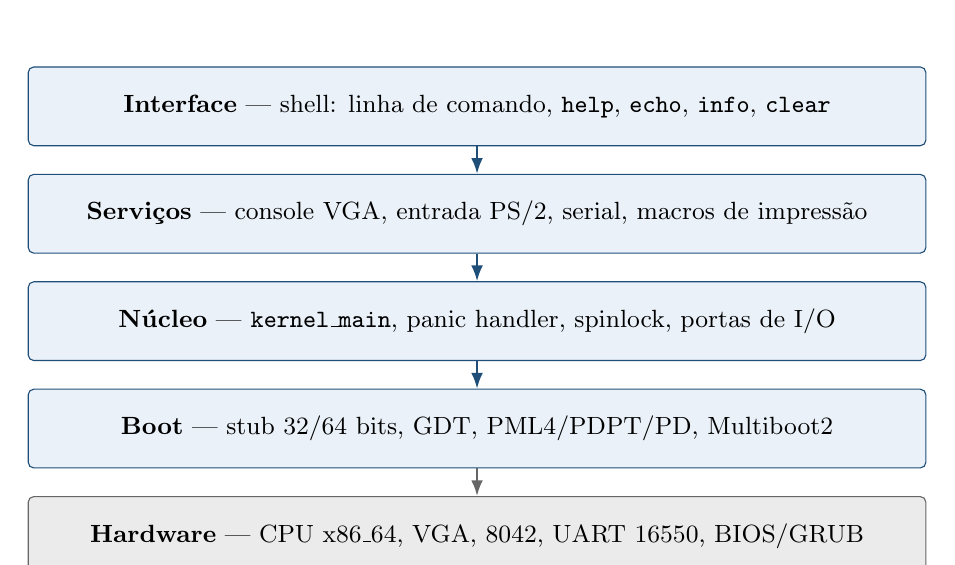
\begin{tikzpicture}[
  layer/.style={draw=rinuxblue, fill=rinuxlight, rounded corners=2pt,
                minimum width=11.4cm, minimum height=1.0cm,
                align=center, font=\small},
  hw/.style={draw=black!60, fill=black!8, rounded corners=2pt,
             minimum width=11.4cm, minimum height=1.0cm,
             align=center, font=\small},
  node distance=0.35cm
]
\node[layer] (shell) {\textbf{Interface} --- shell: linha de comando, \code{help}, \code{echo}, \code{info}, \code{clear}};
\node[layer, below=of shell] (services) {\textbf{Servi\c{c}os} --- console VGA, entrada PS/2, serial, macros de impress\~ao};
\node[layer, below=of services] (core) {\textbf{N\'ucleo} --- \code{kernel\_main}, panic handler, spinlock, portas de I/O};
\node[layer, below=of core] (boot) {\textbf{Boot} --- stub 32/64 bits, GDT, PML4/PDPT/PD, Multiboot2};
\node[hw, below=of boot] (hw) {\textbf{Hardware} --- CPU x86\_64, VGA, 8042, UART 16550, BIOS/GRUB};
\draw[-{Latex[length=2mm]}, thick, rinuxblue] (shell) -- (services);
\draw[-{Latex[length=2mm]}, thick, rinuxblue] (services) -- (core);
\draw[-{Latex[length=2mm]}, thick, rinuxblue] (core) -- (boot);
\draw[-{Latex[length=2mm]}, thick, black!60] (boot) -- (hw);
\end{tikzpicture}
\caption{Camadas do Rust VGA Kernel.}
\label{fig:camadas}
\end{figure}

\section{Modelo de execu\c{c}\~ao}

O kernel executa em \textbf{ring 0}, em uma \'unica CPU, com
\textbf{interrup\c{c}\~oes desligadas}. Todo o processamento \'e feito por
\emph{polling}: o shell consulta o teclado e a serial em um la\c{c}o ativo,
usando \code{core::hint::spin\_loop()} quando n\~ao h\'a entrada.

\begin{table}[H]
\centering
\caption{Caracter\'isticas do modelo de execu\c{c}\~ao.}
\label{tab:modelo}
\begin{tabularx}{\linewidth}{@{}lX@{}}
\toprule
\textbf{Aspecto} & \textbf{Implementa\c{c}\~ao} \\
\midrule
Privil\'egio & Ring 0 \'unico; n\~ao h\'a modo usu\'ario. \\
CPUs & Uma CPU; SMP n\~ao \'e inicializado. \\
Interrup\c{c}\~oes & Desligadas no stub (\code{cli}); nenhuma IDT instalada. \\
Entrada & Polling de \code{0x60}/\code{0x64} e de COM1. \\
Concorr\^encia & Spinlock apenas no console; n\~ao h\'a preemp\c{c}\~ao. \\
Mem\'oria & Est\'atica; sem heap, \code{alloc} ou \code{Vec}. \\
Pilhas & 8 KiB no stub (baixa) e 32 KiB no kernel (alta). \\
Tempo de vida & O shell nunca retorna; \code{halt} e \code{reboot} encerram o fluxo. \\
\bottomrule
\end{tabularx}
\end{table}

\section{Depend\^encias entre m\'odulos}

\begin{figure}[H]
\centering
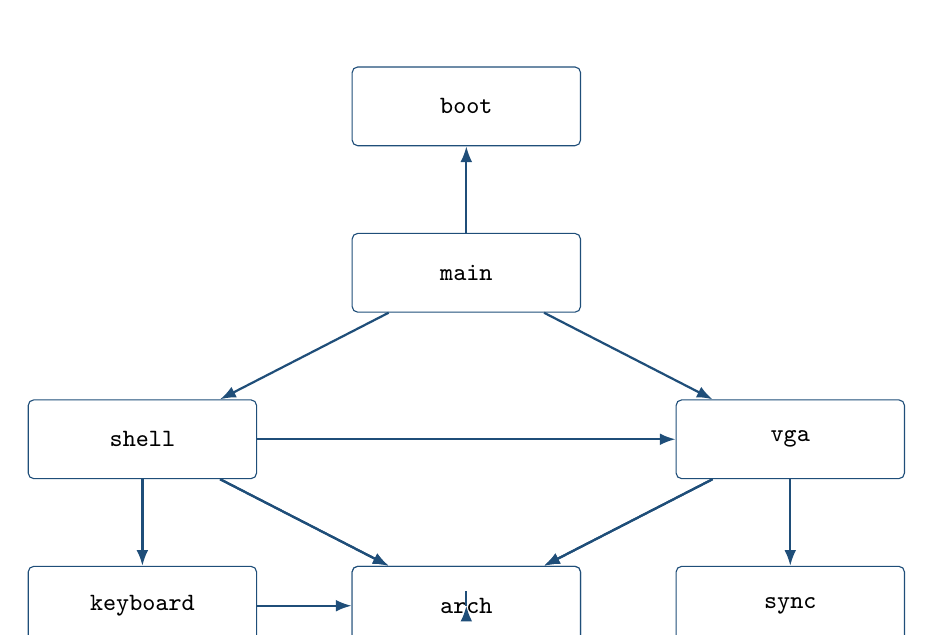
\begin{tikzpicture}[
  mod/.style={draw=rinuxblue, fill=white, rounded corners=2pt,
              minimum width=2.9cm, minimum height=1.0cm,
              align=center, font=\small\ttfamily},
  arrow/.style={-{Latex[length=2mm]}, thick, rinuxblue},
  node distance=1.1cm and 1.2cm
]
\node[mod] (main) {main};
\node[mod, below left=of main] (shell) {shell};
\node[mod, below right=of main] (vga) {vga};
\node[mod, below=of shell] (keyboard) {keyboard};
\node[mod, right=of keyboard] (serial) {serial};
\node[mod, below=of vga] (sync) {sync};
\node[mod, left=of sync] (arch) {arch};
\node[mod, above=of main] (boot) {boot};

\draw[arrow] (main) -- (shell);
\draw[arrow] (main) -- (vga);
\draw[arrow] (main) -- (boot);
\draw[arrow] (shell) -- (keyboard);
\draw[arrow] (shell) -- (serial);
\draw[arrow] (shell) -- (vga);
\draw[arrow] (shell) -- (arch);
\draw[arrow] (vga) -- (serial);
\draw[arrow] (vga) -- (sync);
\draw[arrow] (vga) -- (arch);
\draw[arrow] (keyboard) -- (arch);
\draw[arrow] (serial) -- (arch);
\end{tikzpicture}
\caption{Depend\^encias principais entre m\'odulos. Setas indicam ``usa''.}
\label{fig:dependencias}
\end{figure}

A figura mostra apenas as depend\^encias relevantes. \code{boot.rs} \'e um
caso especial: ele cont\'em o c\'odigo de montagem que chama \code{kernel\_main}
e n\~ao \'e chamado por Rust. \code{main.rs} declara todos os m\'odulos e
exporta as macros \code{print!} e \code{println!}.

\section{Cadeia de boot}

\begin{figure}[H]
\centering
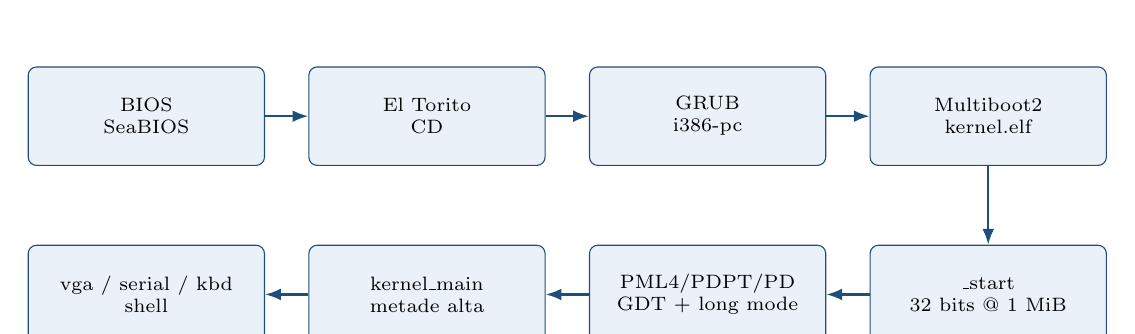
\begin{tikzpicture}[
  stage/.style={draw=rinuxblue, fill=rinuxlight, rounded corners=3pt,
                minimum width=3.0cm, minimum height=1.25cm,
                align=center, font=\scriptsize},
  arrow/.style={-{Latex[length=2mm]}, thick, rinuxblue},
  node distance=0.55cm
]
\node[stage] (bios) {BIOS\\SeaBIOS};
\node[stage, right=of bios] (eltorito) {El Torito\\CD};
\node[stage, right=of eltorito] (grub) {GRUB\\i386-pc};
\node[stage, right=of grub] (mb) {Multiboot2\\kernel.elf};
\node[stage, below=1.0cm of mb] (stub) {\_start\\32 bits @ 1 MiB};
\node[stage, left=of stub] (paging) {PML4/PDPT/PD\\GDT + long mode};
\node[stage, left=of paging] (main) {kernel\_main\\metade alta};
\node[stage, left=of main] (shell) {vga / serial / kbd\\shell};
\draw[arrow] (bios) -- (eltorito);
\draw[arrow] (eltorito) -- (grub);
\draw[arrow] (grub) -- (mb);
\draw[arrow] (mb) -- (stub);
\draw[arrow] (stub) -- (paging);
\draw[arrow] (paging) -- (main);
\draw[arrow] (main) -- (shell);
\end{tikzpicture}
\caption{Cadeia de boot completa.}
\label{fig:bootchain}
\end{figure}

\section{Decis\~oes de projeto}

\begin{table}[H]
\centering
\caption{Decis\~oes arquiteturais e justificativas.}
\label{tab:decisoes}
\begin{tabularx}{\linewidth}{@{}p{3.3cm}X@{}}
\toprule
\textbf{Decis\~ao} & \textbf{Justificativa} \\
\midrule
\code{no\_std} & Elimina depend\^encia de sistema operacional, alocador e
\emph{runtime}; o c\'odigo usa apenas \code{core}. \\
Sem depend\^encias & Reduz superf\'icie de ataque e mant\'em o build
reprodut\'ivel; \code{Cargo.lock} n\~ao tem pacotes externos. \\
Alvo \code{x86\_64-unknown-none} & Alvo oficial bare metal, com modelo de
c\'odigo \emph{kernel} e sem biblioteca padr\~ao. \\
Kernel na metade alta & Conven\c{c}\~ao do Linux e do alvo; evita depender de
endere\c{c}os baixos e deixa o stub separado. \\
Stub em assembly & O controle inicial vem em 32 bits com pilha indefinida;
a transi\c{c}\~ao para 64 bits exige c\'odigo posicional e controle exato. \\
Tabelas de p\'agina est\'aticas & N\~ao h\'a alocador; 3 p\'aginas de 4 KiB
s\~ao suficientes para mapear 1 GiB com \emph{huge pages} de 2 MiB. \\
Polling & Evita IDT, PIC e handlers; simplifica o modelo e mant\'em o foco no
console. \\
Serial al\'em do VGA & Permite depura\c{c}\~ao e testes automatizados sem
depender de captura gr\'afica. \\
\emph{Panic abort} & N\~ao h\'a \emph{unwinding} nem runtime de p\^anico;
\code{panic=abort} reduz c\'odigo gerado. \\
LTO e \code{codegen-units=1} & Gera um bin\'ario pequeno e previs\'ivel; o
linker descarta se\c{c}\~oes n\~ao usadas com \code{--gc-sections}. \\
\bottomrule
\end{tabularx}
\end{table}

\section{Tratamento de erros e falhas}

O kernel n\~ao possui um subsistema de erros. As estrat\'egias s\~ao:

\begin{itemize}
  \item \textbf{Timeout em esperas de hardware}: as fun\c{c}\~oes do 8042
        tentam por um n\'umero limitado de itera\c{c}\~oes e desistem, evitando
        \emph{hang} quando o controlador n\~ao responde.
  \item \textbf{Verifica\c{c}\~ao de presen\c{c}a da UART}: se o registrador de
        status devolver \code{0xFF}, a serial \'e considerada ausente.
  \item \textbf{Entrada inv\'alida}: bytes fora da faixa imprim\'ivel s\~ao
        ignorados no shell; UTF-8 inv\'alido em \code{echo} vira uma
        mensagem fixa.
  \item \textbf{Panic}: o handler imprime \code{[PANIC]} no console e entra em
        \code{halt\_loop()}. Como n\~ao h\'a IDT, uma exce\c{c}\~ao de CPU
        (por exemplo, page fault) causa \emph{triple fault} e reset.
  \item \textbf{Sem recupera\c{c}\~ao}: n\~ao h\'a \emph{kernel oops},
        reinicializa\c{c}\~ao controlada ou despejo de pilha.
\end{itemize}

\section{Concorr\^encia e sincroniza\c{c}\~ao}

Apesar de o sistema ser monoprocessado e rodar com interrup\c{c}\~oes
desligadas, o console \'e protegido por um \code{SpinLock}. Isso permite que
chamadas de impress\~ao vindas de contextos diferentes no futuro n\~ao
intercalem bytes no buffer VGA. O lock usa \code{AtomicBool::swap} com
ordena\c{c}\~ao \code{Acquire} na aquisi\c{c}\~ao e \code{Release} na
libera\c{c}\~ao. A serial n\~ao \'e protegida pelo lock; como o console
escreve VGA e serial em sequ\^encia, uma futura implementa\c{c}\~ao
multithread precisaria de um lock adicional para a UART.

\section{Ciclo de vida da inicializa\c{c}\~ao}

\begin{table}[H]
\centering
\caption{Ordem de inicializa\c{c}\~ao em \code{kernel\_main}.}
\label{tab:init}
\begin{tabular}{@{}clp{7.5cm}@{}}
\toprule
\textbf{\#} & \textbf{Chamada} & \textbf{Efeito} \\
\midrule
1 & \code{vga::init()} & Limpa a tela, zera o cursor, define forma do cursor. \\
2 & \code{serial::init()} & Configura COM1 em 38400 8N1 e detecta presen\c{c}a. \\
3 & \code{keyboard::init()} & Configura o 8042, tradu\c{c}\~ao e varredura. \\
4 & \code{println!} & Banner e mensagem de boas-vindas (VGA + serial). \\
5 & valida\c{c}\~ao & Confere \code{magic == 0x36d76289}. \\
6 & \code{shell::run()} & La\c{c}o eterno de prompt e leitura de comandos. \\
\bottomrule
\end{tabular}
\end{table}

\chapter{Boot e inicializa\c{c}\~ao de baixo n\'ivel}
\label{cap:boot}

\section{Responsabilidades de \code{boot.rs}}

O m\'odulo \code{src/boot.rs} concentra tudo o que precisa acontecer antes de
existir uma pilha Rust, mem\'oria virtual ou console:

\begin{enumerate}
  \item declarar o cabe\c{c}alho Multiboot2 reconhecido pelo GRUB;
  \item salvar os argumentos passados pelo bootloader;
  \item construir as tabelas de p\'agina;
  \item carregar uma GDT de 64 bits;
  \item habilitar PAE, \emph{long mode} e pagina\c{c}\~ao;
  \item transferir o controle para \code{kernel\_main} na metade alta.
\end{enumerate}

O arquivo combina uma estrutura Rust est\'atica (o cabe\c{c}alho) e um bloco
\code{global\_asm!} com o restante. N\~ao h\'a fun\c{c}\~oes Rust nesse
m\'odulo.

\section{Cabe\c{c}alho Multiboot2}

O GRUB procura a assinatura \code{0xE85250D6} nos primeiros 32 KiB do
arquivo. O cabe\c{c}alho \'e declarado em uma \code{static} alinhada a 8 bytes
e colocada na se\c{c}\~ao \code{.multiboot\_header}.

\begin{table}[H]
\centering
\caption{Campos do cabe\c{c}alho Multiboot2 implementado.}
\label{tab:mbheader}
\begin{tabular}{@{}rrl@{}}
\toprule
\textbf{Valor} & \textbf{Offset} & \textbf{Significado} \\
\midrule
\code{0xE85250D6} & 0x00 & Assinatura Multiboot2 \\
\code{0x00000000} & 0x04 & Arquitetura i386 (32 bits) \\
\code{0x00000018} & 0x08 & Tamanho total do cabe\c{c}alho (24 bytes) \\
\code{0x17ADAF12} & 0x0C & Checksum \\
\code{0x00000000} & 0x10 & Tag final: tipo 0 \\
\code{0x00000008} & 0x14 & Tag final: tamanho 8 \\
\bottomrule
\end{tabular}
\end{table}

O checksum \'e calculado de modo que a soma dos quatro primeiros inteiros de
32 bits seja zero:

\begin{verbatim}
-(0xE85250D6 + 0x00000000 + 0x00000018) = 0x17ADAF12
\end{verbatim}

A tag final \'e obrigat\'oria. N\~ao h\'a tags de informa\c{c}\~ao de
v\'ideo, mem\'oria ou m\'odulos; o kernel recebe apenas o ponteiro para a
estrutura Multiboot2 e ignora seu conte\'udo, exceto pelo valor de
\code{magic}, que \'e validado e impresso.

\section{Contrato de entrada}

Quando o GRUB transfere o controle para \code{\_start}:

\begin{itemize}
  \item a CPU est\'a em modo protegido de 32 bits;
  \item \code{eax} cont\'em \code{0x36D76289} (assinatura Multiboot2);
  \item \code{ebx} cont\'em o endere\c{c}o f\'isico da estrutura de
        informa\c{c}\~oes Multiboot2;
  \item a pilha n\~ao \'e confi\'avel;
  \item as interrup\c{c}\~oes podem estar em qualquer estado.
\end{itemize}

O stub imediatamente executa \code{cli} e \code{cld}, define uma pilha
tempor\'aria de 8 KiB em \code{boot\_stack\_top} e zera \code{ebp}.

\section{Sequ\^encia do stub}

\begin{enumerate}
  \item \textbf{Salvar argumentos}: \code{eax} e \code{ebx} s\~ao copiados
        para \code{mb\_magic} e \code{mb\_info}, vari\'aveis de 32 bits em
        \code{.boot.bss}. Como o c\'odigo ainda roda em endere\c{c}os baixos,
        esses endere\c{c}os s\~ao acess\'iveis diretamente.
  \item \textbf{Zerar p\'aginas}: \code{rep stosl} limpa 3 $\times$ 4096
        bytes (PML4, PDPT e PD).
  \item \textbf{Montar PML4}: a entrada 0 aponta para a PDPT e a entrada 511
        tamb\'em aponta para a mesma PDPT. A entrada 511 cobre a faixa
        \code{0xFFFFFF8000000000} em diante.
  \item \textbf{Montar PDPT}: a entrada 0 e a entrada 510 apontam para a
        mesma PD. A entrada 510, dentro do PML4[511], resulta em
        \code{0xFFFFFFFF80000000}.
  \item \textbf{Montar PD}: 512 entradas de 2 MiB, cada uma com os bits
        \emph{present} e \emph{page size} (\code{0x83}),
        mapeando fisicamente 0 a 1 GiB.
  \item \textbf{Carregar GDT}: \code{lgdt gdt64\_ptr}.
  \item \textbf{Preparar a CPU}: limpar \code{CR0.EM}, setar \code{CR0.MP},
        setar \code{CR4.PAE}, \code{CR4.OSFXSR} e \code{CR4.OSXMMEXCPT}.
  \item \textbf{Ativar long mode}: setar \code{EFER.LME} via \code{rdmsr} /
        \code{wrmsr} e, em seguida, \code{CR0.PG | CR0.PE}.
  \item \textbf{Salto de modo}: \code{ljmp \$0x08, \$long\_mode\_entry\_low},
        carregando um seletor de c\'odigo com o bit \code{L} ligado.
  \item \textbf{Modo 64 bits}: recarregar os segmentos de dados com
        \code{0x10}, carregar \code{rsp} com \code{stack\_top} (metade alta),
        preparar \code{edi}/\code{esi} e chamar \code{kernel\_main}.
\end{enumerate}

\begin{nota}[Por que duas pilhas?]
A pilha do stub precisa estar em endere\c{c}o baixo, porque a CPU ainda n\~ao
usa pagina\c{c}\~ao quando o stub come\c{c}a. A pilha definitiva do Rust fica
em \code{.bss}, na metade alta, e s\'o pode ser usada depois que o modo longo
e a pagina\c{c}\~ao est\~ao ativos.
\end{nota}

\section{Pagina\c{c}\~ao e layout de mem\'oria}

A tradu\c{c}\~ao de endere\c{c}os usa quatro n\'iveis, mas apenas tr\^es
tabelas s\~ao preenchidas. O page directory usa \emph{huge pages} de 2 MiB,
reduzindo o consumo a 12 KiB de tabelas.

\begin{figure}[H]
\centering
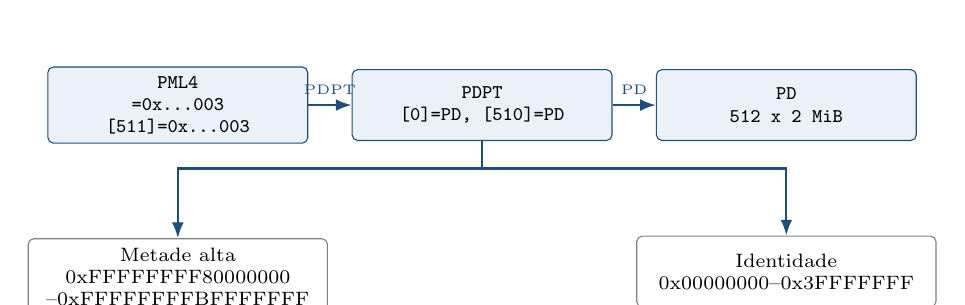
\begin{tikzpicture}[
  tab/.style={draw=rinuxblue, fill=rinuxlight, rounded corners=2pt,
              minimum width=3.3cm, minimum height=0.9cm,
              align=center, font=\scriptsize\ttfamily},
  box/.style={draw=black!50, fill=white, rounded corners=2pt,
              minimum width=3.8cm, minimum height=0.9cm,
              align=center, font=\scriptsize},
  arrow/.style={-{Latex[length=2mm]}, thick, rinuxblue},
  node distance=0.55cm and 0.55cm
]
\node[tab] (pml4) {PML4\\[0]=0x...003\\{[511]=0x...003}};
\node[tab, right=of pml4] (pdpt) {PDPT\\{[0]=PD, [510]=PD}};
\node[tab, right=of pdpt] (pd) {PD\\{512 x 2 MiB}};
\node[box, below=1.2cm of pd] (low) {Identidade\\0x00000000--0x3FFFFFFF};
\node[box, below=1.2cm of pml4] (high) {Metade alta\\0xFFFFFFFF80000000\\--0xFFFFFFFFBFFFFFFF};
\draw[arrow] (pml4) -- node[above,font=\tiny]{PDPT} (pdpt);
\draw[arrow] (pdpt) -- node[above,font=\tiny]{PD} (pd);
\draw[arrow] (pdpt.south) -- ++(0,-0.35) -| (low.north);
\draw[arrow] (pdpt.south) -- ++(0,-0.35) -| (high.north);
\end{tikzpicture}
\caption{Estrutura de pagina\c{c}\~ao: uma \'unica PDPT e uma \'unica PD
servem tanto \`a identidade baixa quanto \`a metade alta.}
\label{fig:paging}
\end{figure}

\subsection{C\'alculo dos \'indices}

Para um endere\c{c}o virtual de 48 bits, os \'indices s\~ao:

\begin{align*}
\text{PML4} &= \left\lfloor \frac{\text{VA}}{2^{39}} \right\rfloor \bmod 512,\\
\text{PDPT} &= \left\lfloor \frac{\text{VA}}{2^{30}} \right\rfloor \bmod 512,\\
\text{PD}   &= \left\lfloor \frac{\text{VA}}{2^{21}} \right\rfloor \bmod 512.
\end{align*}

Para \code{0xFFFFFFFF80000000}:

\begin{itemize}
  \item PML4 = 511 (\code{0xFFFFFFFF80000000 >> 39 \& 0x1FF});
  \item PDPT = 510 (\code{>> 30 \& 0x1FF});
  \item PD = 0.
\end{itemize}

Assim, a entrada 510 da PDPT aponta para a PD que descreve os primeiros 1 GiB
f\'isicos. O mesmo conjunto de tabelas atende aos dois mapeamentos:

\begin{itemize}
  \item \textbf{identidade baixa}: \code{0x00000000}--\code{0x3FFFFFFF}
        (stub, tabelas, estruturas do GRUB);
  \item \textbf{metade alta}: \code{0xFFFFFFFF80000000}--
        \code{0xFFFFFFFFBFFFFFFF} (c\'odigo e dados do kernel).
\end{itemize}

\begin{atencao}[Limite de 1 GiB]
O mapeamento cobre exatamente 1 GiB. Se o kernel ou o \emph{framebuffer}
estiverem acima disso, ou se a m\'aquina tiver mais de 1 GiB e o kernel
precisar acessar mem\'oria al\'em desse limite, o mapeamento precisa ser
estendido (mais entradas na PD ou tabelas adicionais).
\end{atencao}

\section{GDT e modo longo}

A GDT cont\'em tr\^es descritores:

\begin{table}[H]
\centering
\caption{Descritores da GDT de 64 bits.}
\label{tab:gdt}
\begin{tabular}{@{}clll@{}}
\toprule
\textbf{Seletor} & \textbf{Valor} & \textbf{Tipo} & \textbf{Uso} \\
\midrule
\code{0x00} & \code{0x0000000000000000} & Nulo & Obrigat\'orio \\
\code{0x08} & \code{0x00AF9A000000FFFF} & C\'odigo ring 0, L=1 & \code{CS} \\
\code{0x10} & \code{0x00CF92000000FFFF} & Dados ring 0 & \code{DS/ES/FS/GS/SS} \\
\bottomrule
\end{tabular}
\end{table}

O descritor de c\'odigo tem o bit \code{L} (long mode) ligado, indicando
c\'odigo de 64 bits. O descritor de dados \'e o tradicional de 32 bits, usado
apenas para os registradores de segmento; em modo longo, a segmenta\c{c}\~ao
de dados \'e praticamente ignorada.

\section{Registradores de controle}

\begin{table}[H]
\centering
\caption{Configura\c{c}\~ao dos registradores de controle.}
\label{tab:cr}
\begin{tabular}{@{}llp{7.5cm}@{}}
\toprule
\textbf{Registrador} & \textbf{Bits} & \textbf{Efeito} \\
\midrule
\code{CR0} & \code{EM=0}, \code{MP=1} & Habilita SSE/FXSR sem emula\c{c}\~ao de FPU. \\
\code{CR0} & \code{PG=1}, \code{PE=1} & Ativa pagina\c{c}\~ao e modo protegido. \\
\code{CR3} & \code{pml4} & Aponta para o PML4 f\'isico. \\
\code{CR4} & \code{PAE=1} & Habilita endere\c{c}os f\'isicos de 36 bits e p\'aginas de 2 MiB. \\
\code{CR4} & \code{OSFXSR=1} & Sistema operacional suporta \code{FXSAVE}/\code{FXRSTOR}. \\
\code{CR4} & \code{OSXMMEXCPT=1} & Exce\c{c}\~oes SIMD entregues ao SO. \\
\code{EFER} & \code{LME=1} & Habilita \emph{long mode}. \\
\bottomrule
\end{tabular}
\end{table}

\section{Linker script}

O arquivo \code{linker.ld} define dois mundos:

\begin{enumerate}
  \item \code{.boot}, carregado em \code{0x100000} (1 MiB), cont\'em o
        cabe\c{c}alho Multiboot2, o c\'odigo de 32/64 bits, a GDT, as tabelas
        de p\'agina e a pilha do stub;
  \item \code{.text}, \code{.rodata}, \code{.data} e \code{.bss}, ligados em
        \code{0xFFFFFFFF80000000} com \emph{load address} f\'isico
        \code{0x00100000 + deslocamento}.
\end{enumerate}

A macro \code{KERNEL\_VMA} vale \code{0xFFFFFFFF80000000}. Para cada
se\c{c}\~ao alta, o script usa \code{AT(ADDR(.secao) - KERNEL\_VMA)} para
informar ao linker que o endere\c{c}o de carga f\'isico \'e baixo, embora o
endere\c{c}o virtual seja alto.

\begin{lstlisting}[caption={Trecho central de \code{linker.ld}.},label={lst:linker}]
ENTRY(_start)
KERNEL_VMA = 0xFFFFFFFF80000000;

SECTIONS
{
    . = 1M;

    .boot : ALIGN(8)
    {
        KEEP(*(.multiboot_header))
        *(.text.boot)
        *(.boot.rodata)
        *(.boot.data)
        *(.boot.bss)
    }

    . = ALIGN(4096);
    . += KERNEL_VMA;

    .text : AT(ADDR(.text) - KERNEL_VMA)
    {
        *(.text .text.*)
    }
    /* .rodata, .data e .bss seguem o mesmo padrao */
}
\end{lstlisting}

Se\c{c}\~oes de metadados que n\~ao s\~ao necess\'arias em um kernel
(\code{.eh\_frame}, \code{.comment}, \code{.note}) s\~ao descartadas com
\code{/DISCARD/}, e o build usa \code{--gc-sections} para remover c\'odigo
n\~ao referenciado.

\section{Se\c{c}\~oes observadas no ELF}

A compila\c{c}\~ao de refer\^encia gerou o seguinte layout:

\begin{table}[H]
\centering
\caption{Se\c{c}\~oes do ELF de refer\^encia (endere\c{c}os virtuais).}
\label{tab:elf}
\begin{tabular}{@{}llrr@{}}
\toprule
\textbf{Se\c{c}\~ao} & \textbf{VMA} & \textbf{Offset} & \textbf{Tamanho} \\
\midrule
\code{.boot}   & \code{0x0000000000100000} & \code{0x1000} & \code{0x6008} \\
\code{.text}   & \code{0xFFFFFFFF80107000} & \code{0x8000} & \code{0x2516} \\
\code{.rodata} & \code{0xFFFFFFFF80109518} & \code{0xA518} & \code{0x0AE7} \\
\code{.data}   & \code{0xFFFFFFFF8010A000} & \code{0xB000} & \code{0x0020} \\
\code{.bss}    & \code{0xFFFFFFFF8010A020} & \code{0xB020} & \code{0x8003} \\
\bottomrule
\end{tabular}
\end{table}

O ponto de entrada \'e \code{0x100018}, dentro de \code{.boot}. O ELF tem
6 \emph{program headers}: um segmento baixo \code{RWE} para o stub e quatro
segmentos altos (c\'odigo, read-only, dados e BSS).

\section{Passagem para Rust}

O \'ultimo trecho do stub carrega os argumentos e chama a fun\c{c}\~ao Rust:

\begin{lstlisting}[caption={Chamada de \code{kernel\_main} a partir do stub.},label={lst:callmain}]
    mov mb_magic(%rip), %edi
    mov mb_info(%rip), %esi
    movabs $kernel_main, %rax
    call *%rax

3:
    cli
    hlt
    jmp 3b
\end{lstlisting}

A fun\c{c}\~ao Rust usa a conven\c{c}\~ao \code{extern "C"}: os dois primeiros
argumentos inteiros v\~ao em \code{edi} e \code{esi}. O retorno \'e
\code{!}, mas o stub ainda mant\'em um la\c{c}o de seguran\c{c}a com
\code{cli; hlt} caso a chamada retorne inesperadamente.

\section{Limita\c{c}\~oes do boot}

\begin{itemize}
  \item N\~ao h\'a suporte a UEFI nativo; depende de BIOS/CSM e de VGA
        legado.
  \item N\~ao h\'a real-mode setup, \emph{protected mode} pr\'oprio nem
        descompress\~ao; o GRUB faz o carregamento.
  \item O cabe\c{c}alho n\~ao solicita informa\c{c}\~oes de mem\'oria,
        framebuffer ou m\'odulos; a estrutura Multiboot2 n\~ao \'e
        interpretada al\'em do \code{magic}.
  \item Apenas 1 GiB \'e mapeado e n\~ao h\'a \emph{demand paging},
        prote\c{c}\~ao \code{NX}, \emph{user/kernel} ou \emph{guard pages}.
  \item Sem IDT, qualquer exce\c{c}\~ao (incluindo \emph{page fault})
        resulta em \emph{triple fault}.
\end{itemize}

\chapter{Base modules}
\label{cap:base}

This chapter documents the modules that do not belong to a specific driver:
\code{main.rs}, \code{arch.rs}, and \code{sync.rs}. They provide the entry
point, the printing macros, I/O port access,
shutdown/reboot, and the console spinlock.

\section{\code{main.rs}: Rust entry point}

\subsection{Global attributes}

\begin{lstlisting}[caption={Attributes and modules declared in \code{main.rs}.},label={lst:mainattrs}]
#![no_std]
#![no_main]

mod arch;
mod boot;
mod gdt;
mod idt;
mod keyboard;
mod paging;
mod serial;
mod shell;
mod sync;
mod user;
mod vga;
\end{lstlisting}

\begin{itemize}
  \item \code{no\_std}: the crate does not use the standard library; there is no
        \code{std::io}, \code{String}, \code{Vec}, filesystem, or
        \emph{threads}.
  \item \code{no\_main}: the Rust runtime \code{main} function does not exist.
        The real entry point is \code{\_start}, defined in the
        assembly of \code{boot.rs}.
  \item \code{mod boot}: required for the linker to include the assembly code
        and the Multiboot2 header.
\end{itemize}

\subsection{\code{kernel\_main}}

\begin{lstlisting}[caption={Signature and main body of \code{kernel\_main}.},label={lst:kernelmain}]
#[unsafe(no_mangle)]
pub extern "C" fn kernel_main(multiboot_magic: u32, multiboot_info: u32) -> ! {
    vga::init();
    serial::init();
    paging::init(multiboot_magic, multiboot_info);
    gdt::init();
    keyboard::init();
    idt::init();
    arch::enable_interrupts();

    println!();
    println!("==============================================================");
    println!("  Rust VGA Kernel - x86_64 / modo longo");
    /* ... banner ... */

    if multiboot_magic != 0x36d7_6289 {
        println!("AVISO: assinatura multiboot2 invalida: {:#010x}",
                 multiboot_magic);
    }
    println!("Multiboot2: magic={:#010x} info={:#010x}",
             multiboot_magic, multiboot_info);
    println!();
    println!("Digite 'help' para ver os comandos.");
    println!();

    shell::run()
}
\end{lstlisting}

\begin{table}[H]
\centering
\caption{Contract of \code{kernel\_main}.}
\label{tab:kernelmain}
\begin{tabularx}{\linewidth}{@{}lX@{}}
\toprule
\textbf{Aspect} & \textbf{Description} \\
\midrule
Visibility & \code{pub extern "C"}, exported without \emph{mangling}. \\
Arguments & \code{multiboot\_magic} (must be \code{0x36D76289}) and
\code{multiboot\_info} (physical address of the Multiboot2 structure). \\
Return & \code{!}: never returns; ends in \code{shell::run()}. \\
Preconditions & CPU in long mode, paging active, valid higher-half
stack, \code{.bss} zeroed by the loader. \\
Effects & Initializes VGA, serial, frame allocator, GDT/TSS, keyboard,
IDT/PIC/PIT, and enables interrupts; prints the banner; enters the shell. \\
Called by & Assembly stub in \code{boot.rs}. \\
\bottomrule
\end{tabularx}
\end{table}

The \code{multiboot\_info} value is used by \code{paging::init} to
walk the Multiboot2 tags and free the available RAM frames. The
structure is also reserved so that it is not handed out by the allocator.

\subsection{\code{print!} and \code{println!} macros}

The macros are defined with \code{macro\_rules!} and \code{\$crate}, so that
they work in any module of the crate without imports:

\begin{lstlisting}[caption={Printing macros without allocation.},label={lst:macros}]
#[macro_export]
macro_rules! print {
    ($($arg:tt)*) => {
        $crate::vga::_print(format_args!($($arg)*))
    };
}

#[macro_export]
macro_rules! println {
    () => { $crate::print!("\n") };
    ($($arg:tt)*) => {
        $crate::print!("{}\n", format_args!($($arg)*))
    };
}
\end{lstlisting}

\code{format\_args!} creates a formatting description without allocating;
the \code{fmt::Write} implementation in \code{vga.rs} consumes the
fragments. There is no \code{format!} (which would require \code{alloc}).

\subsection{Panic handler}

\begin{lstlisting}[caption={\emph{Panic handler} of the kernel.},label={lst:panic}]
#[panic_handler]
fn panic(info: &PanicInfo) -> ! {
    crate::println!();
    crate::println!("[PANIC] {}", info);
    crate::arch::halt_loop()
}
\end{lstlisting}

Because the profile uses \code{panic = "abort"}, the handler does not need
\emph{unwinding}. It prints the message to the console and halts the CPU. If the
panic occurs before \code{vga::init()}, the output may not be
visible; if it occurs inside the console with the spinlock held, a
\emph{deadlock} may occur (the handler would try to print and would wait for the lock).

\section{\code{arch.rs}: architecture and I/O ports}

\subsection{I/O ports}

The \code{arch::port} module encapsulates the x86 \code{in} and
\code{out} instructions:

\begin{lstlisting}[caption={Reading and writing 8-bit ports.},label={lst:portio}]
pub unsafe fn inb(port: u16) -> u8 {
    let value: u8;
    asm!("in al, dx",
         in("dx") port,
         out("al") value,
         options(nomem, nostack, preserves_flags));
    value
}

pub unsafe fn outb(port: u16, value: u8) {
    asm!("out dx, al",
         in("dx") port,
         in("al") value,
         options(nomem, nostack, preserves_flags));
}
\end{lstlisting}

The functions are \code{unsafe} because any port may not exist
or may have side effects on the hardware. The \code{nomem},
\code{nostack}, and \code{preserves\_flags} options tell the compiler that the
instruction does not change memory, stack, or flags, allowing optimizations
and preventing the block from being removed.

\begin{table}[H]
\centering
\caption{API of \code{arch}.}
\label{tab:archapi}
\begin{tabularx}{\linewidth}{@{}lX@{}}
\toprule
\textbf{Function} & \textbf{Description} \\
\midrule
\code{inb(port)} & Reads a byte from an I/O port. \code{unsafe}. \\
\code{outb(port, value)} & Writes a byte to a port. \code{unsafe}. \\
\code{halt\_loop()} & Executes \code{cli; hlt} in an infinite loop; does not
return. Used in the panic handler and in the \code{halt} command. \\
\code{reboot()} & Waits for the 8042 input buffer to empty and sends the
\code{0xFE} command (reset). If it does not work, it falls back to \code{halt\_loop}. \\
\bottomrule
\end{tabularx}
\end{table}

\subsection{Reboot}

The reset uses the 8042 controller, which historically controls the CPU reset
line. The code waits up to 100,000 iterations for the
\code{INPUT\_FULL} bit (\code{0x02}) of the status register to clear and writes \code{0xFE} to the
command port (\code{0x64}). On virtualized machines or machines without an 8042, the
reset may not occur; in that case the CPU is halted.

\section{\code{sync.rs}: spinlock}

\subsection{Implementation}

\begin{lstlisting}[caption={Spinlock with \code{AtomicBool}.},label={lst:spinlock}]
pub struct SpinLock<T> {
    locked: AtomicBool,
    data: UnsafeCell<T>,
}

unsafe impl<T: Send> Sync for SpinLock<T> {}
unsafe impl<T: Send> Send for SpinLock<T> {}

impl<T> SpinLock<T> {
    pub const fn new(data: T) -> Self { /* ... */ }

    pub fn lock(&self) -> SpinLockGuard<'_, T> {
        while self.locked.swap(true, Ordering::Acquire) {
            core::hint::spin_loop();
        }
        SpinLockGuard { lock: self }
    }
}
\end{lstlisting}

The \emph{guard} implements \code{Deref}, \code{DerefMut}, and \code{Drop}. When it is
destroyed, it stores \code{false} with \code{Release} ordering. The
spinlock is used only for the console:

\begin{lstlisting}[caption={Global console protected by a spinlock.},label={lst:consoleglobal}]
static CONSOLE: SpinLock<Console> = SpinLock::new(Console::new());
\end{lstlisting}

Because \code{Console::new()} is \code{const}, the lock can be initialized
statically without runtime initialization code.

\subsection{Properties and limitations}

\begin{itemize}
  \item \textbf{Spinning lock}: if another CPU or an interrupt
        holds the lock, the current CPU spins until it is released. There is no
        \emph{sleep} or timeout.
  \item \textbf{No IRQ save/restore}: disabling interrupts when
        acquiring the lock is not done. With IRQs disabled at boot, this is
        not a problem today; once IRQs are enabled, a handler that uses the
        console may cause a \emph{deadlock}.
  \item \textbf{No recursion detection}: acquiring the same lock twice
        on the same CPU hangs.
  \item \textbf{Memory ordering}: \code{Acquire}/\code{Release} guarantees
        that writes to the console are not reordered out of the
        critical section on architectures with weak memory; on x86,
        the model is stronger, but the annotation keeps the code
        correct.
\end{itemize}

\begin{nota}[Current scope]
With one CPU, interrupts disabled, and only the shell calling
\code{print!}, the spinlock is never contended. It exists as preparation
for extensions and to document the intent of mutual exclusion.
\end{nota}

\chapter{VGA console in text mode}
\label{cap:vga}

\section{Overview}

The \code{src/vga.rs} driver is the simplified equivalent of Linux's
\code{vgacon}. It operates in the legacy VGA text mode, in which the screen is an
80-column by 25-row matrix stored starting from the physical address
\code{0xB8000}. Each cell occupies 16 bits.

\begin{table}[H]
\centering
\caption{Format of a VGA text cell.}
\label{tab:vgacell}
\begin{tabular}{@{}lll@{}}
\toprule
\textbf{Bits} & \textbf{Field} & \textbf{Value used} \\
\midrule
0--7  & ASCII character & Character code \\
8--11 & Foreground color & \code{0x7} (light gray) \\
12--14 & Background color & \code{0x0} (black) \\
15    & Blink & \code{0} (off) \\
\midrule
\multicolumn{3}{@{}l@{}}{\textbf{Full attribute}: \code{0x07}} \\
\bottomrule
\end{tabular}
\end{table}

The buffer has $80 \times 25 = 2{,}000$ cells, or 4,000 bytes. The cursor
position is controlled by the CRTC registers, accessed through ports
\code{0x3D4} (index) and \code{0x3D5} (data).

\section{Console state}

\begin{lstlisting}[caption={State maintained by the console.},label={lst:consolestate}]
struct Console {
    column: usize,
    row: usize,
    color: u8,
}
\end{lstlisting}

The state is protected by \code{static CONSOLE: SpinLock<Console>}. There is
no \emph{scrollback} buffer, nor memory separate from the screen: each
change is written directly to the \emph{framebuffer} with
\code{write\_volatile}.

\section{Operations}

\subsection{Initialization}

\code{vga::init()}:

\begin{enumerate}
  \item acquires the console lock;
  \item fills the 2,000 cells with a space and the \code{0x07} attribute;
  \item zeroes the column and row;
  \item configures the cursor as a bottom line, writing
        \code{0x0E} to register \code{0x0A} (cursor start) and
        \code{0x0F} to register \code{0x0B} (cursor end);
  \item updates the cursor position.
\end{enumerate}

\subsection{Byte output}

\begin{lstlisting}[caption={Handling of control and printable characters.},label={lst:writebyte}]
fn write_byte(&mut self, byte: u8) {
    match byte {
        b'\n' => self.newline(),
        b'\r' => { self.column = 0; self.update_cursor(); }
        b'\t' => {
            let next = (self.column + 8) & !7;
            if next >= BUFFER_WIDTH { self.newline(); }
            else { self.column = next; self.update_cursor(); }
        }
        0x08 => self.backspace(),
        0x20..=0x7E => self.write_char(byte as char),
        _ => self.write_char('?'),
    }
}
\end{lstlisting}

Printable ASCII characters are written directly. Any other
byte becomes \code{?}; this includes UTF-8 accented characters, which arrive as
individual bytes and are not decoded.

\subsection{Character output and line break}

\code{write\_char}:

\begin{itemize}
  \item if the column is at 80, it calls \code{newline()};
  \item computes the index \code{row * 80 + column};
  \item writes \code{(ch as u16) | (color << 8)} with \code{write\_volatile};
  \item increments the column;
  \item if the column has reached 80, it calls \code{newline()}; otherwise,
        it updates the cursor.
\end{itemize}

\code{newline()} zeroes the column and increments the row. If the current row is the
last one (24), it calls \code{scroll()}.

\subsection{Scrolling}

\code{scroll()} moves each cell from row $n$ to row $n-1$ and clears the
last row. The algorithm is $O(80 \times 24)$ per additional row and does not
use temporary memory:

\begin{lstlisting}[caption={Core of the scrolling.},label={lst:scroll}]
for row in 1..BUFFER_HEIGHT {
    for column in 0..BUFFER_WIDTH {
        let src = row * BUFFER_WIDTH + column;
        let dst = (row - 1) * BUFFER_WIDTH + column;
        let cell = read_volatile(VGA_BUFFER.add(src));
        write_volatile(VGA_BUFFER.add(dst), cell);
    }
}
/* limpa a ultima linha */
\end{lstlisting}

Because source and destination overlap and the copy is done from top to bottom,
there is no loss of cells that have not yet been copied.

\subsection{Backspace}

Backspace moves the column back; if it is at column 0, it moves to the end of the
previous row. It then writes a blank cell at the position and updates
the cursor. It does not erase beyond position (0,0).

\subsection{Hardware cursor}

The position is computed as \code{row * 80 + column} and split into two
bytes:

\begin{lstlisting}[caption={Cursor update via CRTC.},label={lst:cursor}]
outb(0x3D4, 0x0F);
outb(0x3D5, (position & 0xFF) as u8);
outb(0x3D4, 0x0E);
outb(0x3D5, (position >> 8) as u8);
\end{lstlisting}

Register \code{0x0E} receives the high byte and \code{0x0F} the low byte.

\section{Printing pipeline}

\begin{figure}[H]
\centering
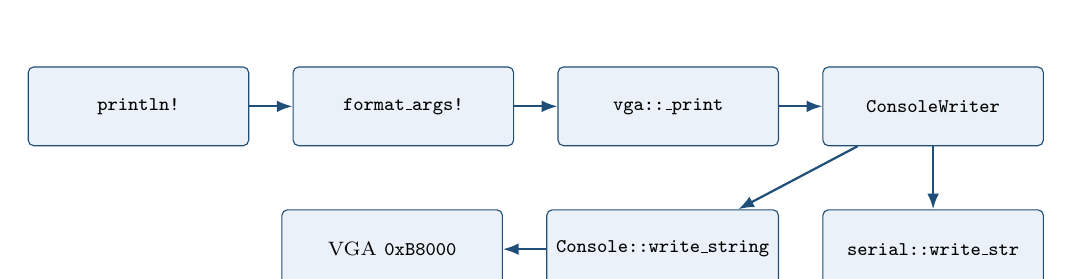
\begin{tikzpicture}[
  box/.style={draw=rinuxblue, fill=rinuxlight, rounded corners=2pt,
              minimum width=2.8cm, minimum height=1.0cm,
              align=center, font=\scriptsize},
  arrow/.style={-{Latex[length=2mm]}, thick, rinuxblue},
  node distance=0.55cm
]
\node[box] (macro) {\code{println!}};
\node[box, right=of macro] (args) {\code{format\_args!}};
\node[box, right=of args] (print) {\code{vga::\_print}};
\node[box, right=of print] (writer) {\code{ConsoleWriter}};
\node[box, below=0.8cm of writer] (serial) {\code{serial::write\_str}};
\node[box, left=of serial] (vga) {\code{Console::write\_string}};
\node[box, left=of vga] (fb) {VGA \code{0xB8000}};
\draw[arrow] (macro) -- (args);
\draw[arrow] (args) -- (print);
\draw[arrow] (print) -- (writer);
\draw[arrow] (writer) -- (vga);
\draw[arrow] (writer) -- (serial);
\draw[arrow] (vga) -- (fb);
\end{tikzpicture}
\caption{Flow of a print call: VGA and serial receive the same text.}
\label{fig:printpipeline}
\end{figure}

\code{ConsoleWriter} implements \code{fmt::Write}. It acquires the lock,
writes to VGA, releases the lock, and only then writes to serial. This avoids
holding the lock while waiting for the UART.

\section{Public API}

\begin{table}[H]
\centering
\caption{Functions and constants of \code{vga.rs}.}
\label{tab:vgaapi}
\begin{tabularx}{\linewidth}{@{}lX@{}}
\toprule
\textbf{Item} & \textbf{Description} \\
\midrule
\code{BUFFER\_WIDTH = 80} & Screen columns. \\
\code{BUFFER\_HEIGHT = 25} & Screen rows. \\
\code{init()} & Clears the screen, configures the cursor shape and position. \\
\code{clear()} & Clears the screen (\code{clear} command). \\
\code{\_print(args)} & Entry point of the macros; writes to VGA and serial. \\
\code{Console::clear()} & Fills the buffer and repositions the cursor. \\
\code{Console::write\_byte()} & Interprets controls and characters. \\
\code{Console::write\_char()} & Writes a cell and advances the column. \\
\code{Console::write\_string()} & Iterates over the bytes of a \code{\&str}. \\
\code{Console::newline()} & Advances the row, scrolling if necessary. \\
\code{Console::backspace()} & Moves back and erases a cell. \\
\code{Console::scroll()} & Moves the content up by one row. \\
\code{Console::update\_cursor()} & Writes the position to the CRTC. \\
\bottomrule
\end{tabularx}
\end{table}

\section{Usage example}

\begin{lstlisting}[caption={Use of the macros in the shell.},label={lst:usovga}]
crate::print!("rinux> ");
println!("Comandos disponiveis:");
crate::print!("\x08");
\end{lstlisting}

The first command prints the prompt without a line break. The second prints
a complete line. The third sends the backspace character to erase the
last visible character.

\section{Limitations and observations}

\begin{itemize}
  \item \textbf{VGA text only}: there is no graphics framebuffer, VBE,
        GOP, or virtual console (VT). On UEFI without CSM, \code{0xB8000} may
        not exist.
  \item \textbf{ASCII only}: there is no UTF-8 decoding or
        built-in bitmap font; the font comes from VGA.
  \item \textbf{No dynamic attributes}: \code{color} exists in the state,
        but there is no public API to change it.
  \item \textbf{No synchronization with vertical retrace}: writes
        may cause occasional \emph{tearing}, irrelevant for text.
  \item \textbf{No memory protection}: \code{0xB8000} is accessed
        as a raw pointer; an invalid address would cause a fault.
  \item \textbf{Unchecked index}: \code{row} and \code{column}
        are kept within bounds by the functions, but there is no
        \emph{assert} of invariants.
  \item \textbf{Scroll costs 1,920 reads/writes}: acceptable for a
        terminal, but it could use \emph{hardware scrolling} or intermediate
        memory.
\end{itemize}

\chapter{PS/2 Keyboard}
\label{cap:keyboard}

\section{Overview}

The \code{src/keyboard.rs} driver implements the subset needed to read keys
from a PS/2 keyboard connected to the 8042 controller. It combines concepts
from two Linux subsystems:

\begin{itemize}
  \item \code{drivers/input/serio/i8042.c}: controller access and the command
        protocol;
  \item \code{drivers/input/keyboard/atkbd.c}: scancode and modifier key
        interpretation.
\end{itemize}

There is no IRQ1, event queue, \code{input\_device}, Linux \emph{keycode}, or
\code{evdev}. The driver does \emph{polling} of the 8042 output buffer and
returns either an ASCII character or a console switch request to the TTY
layer.

\section{Hardware: 8042 controller}

The 8042 exposes two ports:

\begin{table}[H]
\centering
\caption{Ports of the 8042 controller.}
\label{tab:ports8042}
\begin{tabular}{@{}lll@{}}
\toprule
\textbf{Port} & \textbf{Name} & \textbf{Usage} \\
\midrule
\code{0x60} & Data & Reading scancodes; writing data to the keyboard. \\
\code{0x64} & Status/Command & Reading status; writing commands to the 8042. \\
\bottomrule
\end{tabular}
\end{table}

The status register (\code{0x64}) has the bits used by the driver:

\begin{table}[H]
\centering
\caption{8042 status bits.}
\label{tab:status8042}
\begin{tabular}{@{}lll@{}}
\toprule
\textbf{Bit} & \textbf{Mask} & \textbf{Meaning} \\
\midrule
0 & \code{0x01} & Output buffer full (there is data to read) \\
1 & \code{0x02} & Input buffer full (do not send a command) \\
5 & \code{0x20} & Data came from the auxiliary device (mouse) \\
\bottomrule
\end{tabular}
\end{table}

\section{Initialization}

Initialization is more than clearing the buffer. The BIOS or GRUB may leave
the controller in a state where the keyboard sends set 2 scancodes, while the
driver expects set 1, or with scanning disabled. The procedure implemented is:

\begin{table}[H]
\centering
\caption{8042 initialization sequence.}
\label{tab:kbdinit}
\begin{tabular}{@{}clp{7.3cm}@{}}
\toprule
\textbf{\#} & \textbf{Command} & \textbf{Effect} \\
\midrule
1 & reads from \code{0x60} & Discards pending bytes in the output buffer. \\
2 & \code{0xAD} in \code{0x64} & Disables the keyboard port. \\
3 & \code{0x20} in \code{0x64} & Requests a read of the \emph{configuration byte}. \\
4 & read from \code{0x60} & Obtains the current configuration byte
(or uses \code{0x45} if there is no response). \\
5 & adjustment & Turns on translation (bit 6), turns off IRQ1 (bit 0), and
turns on the clock (clears bit 4). \\
6 & \code{0x60} in \code{0x64} & Prepares the write of the new configuration
byte. \\
7 & byte in \code{0x60} & Sends the new \emph{configuration byte}. \\
8 & \code{0xAE} in \code{0x64} & Re-enables the keyboard port. \\
9 & \code{0xF4} in \code{0x60} & Sends the \emph{enable scanning} command to
the keyboard. \\
10 & read from \code{0x60} & Consumes the ACK (\code{0xFA}), if present. \\
11 & cleanup & Discards any residue from the buffer. \\
\bottomrule
\end{tabular}
\end{table}

\begin{nota}[Why translate?]
The modern PS/2 keyboard usually speaks \emph{scan code set 2}, but the 8042
controller can present \emph{set 1} to the system when the translation bit is
on. Linux also configures this translation in i8042. Without it, keys arrive in
codes different from those expected by the driver's table.
\end{nota}

The waits use up to 100,000 iterations, both for the input buffer to empty and
for the output buffer to fill. If the controller does not respond,
initialization continues instead of hanging.

\section{Scancodes and ASCII translation}

The driver works with set 1. The \code{KEYMAP} table has 128 positions and
covers letters, digits, space, and some symbols. Unmapped positions are zero
and are ignored.

\begin{table}[H]
\centering
\caption{Examples of set 1 scancodes.}
\label{tab:scancodes}
\begin{tabular}{@{}llll@{}}
\toprule
\textbf{Key} & \textbf{Make} & \textbf{Break} & \textbf{Result} \\
\midrule
\code{A} & \code{0x1E} & \code{0x9E} & \code{a} / \code{A} with Shift \\
\code{1} & \code{0x02} & \code{0x82} & \code{1} / \code{!} with Shift \\
\code{Enter} & \code{0x1C} & \code{0x9C} & \code{\textbackslash n} \\
\code{Backspace} & \code{0x0E} & \code{0x8E} & \code{0x08} \\
\code{Tab} & \code{0x0F} & \code{0x8F} & \code{\textbackslash t} \\
\code{Space} & \code{0x39} & \code{0xB9} & space \\
\code{Left Shift} & \code{0x2A} & \code{0xAA} & enables/disables Shift \\
\code{Right Shift} & \code{0x36} & \code{0xB6} & enables/disables Shift \\
\code{Left Alt} & \code{0x38} & \code{0xB8} & enables/disables Alt \\
\code{F1}..\code{F8} & \code{0x3B}..\code{0x42} & \code{0xBB}..\code{0xC2}
& \code{Alt+F1}..\code{Alt+F8} selects \code{tty0}..\code{tty7} \\
\code{Extended key} & \code{0xE0} & --- & prefix; next code ignored \\
\bottomrule
\end{tabular}
\end{table}

\subsection{Shift}

The Shift state is kept in \code{static SHIFT: AtomicBool}. The \code{0x2A}
and \code{0x36} keys turn the state on; the \emph{break codes} \code{0xAA} and
\code{0xB6} turn it off. The \code{apply\_shift} function transforms letters to
uppercase and applies the secondary symbol of digits and punctuation:

\begin{lstlisting}[caption={Mapping with Shift.},label={lst:shift}]
b'a'..=b'z' => byte - 32,
b'1'..=b'9' => b"!@#$%^&*("[(byte - b'1') as usize],
b'0' => b')',
b'-' => b'_',
b'=' => b'+',
/* ... */
\end{lstlisting}

\subsection{Extended keys}

The \code{0xE0} prefix sets the \code{EXTENDED} flag. The next scancode is
discarded and the flag is cleared. This prevents arrows, Insert, Delete, Home,
End, and numeric keypad keys from being interpreted as letters. The
consequence is that these keys have no function in the shell.

\subsection{Alt and console selection}

The Alt state is kept in \code{static ALT: AtomicBool}: scancode \code{0x38}
sets it and the break code \code{0xB8} clears it. While Alt is held, the F1
through F8 scancodes (\code{0x3B}..\code{0x42}) are not translated to ASCII.
They produce \code{Key::Console(0..7)}, which the TTY layer uses to switch to
\code{tty0}..\code{tty7}.

\begin{lstlisting}[caption={Result of the keyboard driver.},label={lst:key}]
pub enum Key {
    Char(u8),
    Console(usize),
}
\end{lstlisting}

\subsection{Mouse}

Mouse data shares the same 8042. If bit 5 of the status is on, the byte read
is discarded. This prevents mouse movements from appearing as letters.

\section{Read flow}

\begin{figure}[H]
\centering
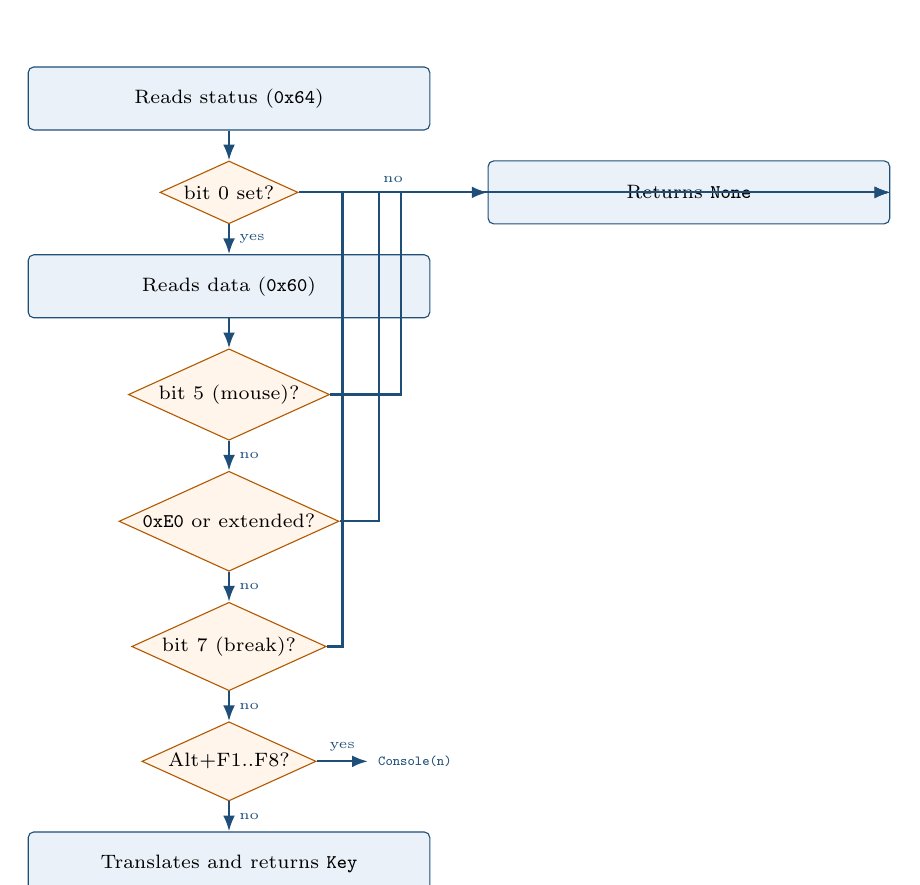
\begin{tikzpicture}[
  kstep/.style={draw=rinuxblue, fill=rinuxlight, rounded corners=2pt,
               minimum width=5.1cm, minimum height=0.8cm,
               align=center, font=\scriptsize},
  dec/.style={draw=orange!70!black, fill=orange!8, diamond, aspect=2.2,
              inner sep=1pt, align=center, font=\scriptsize},
  arrow/.style={-{Latex[length=2mm]}, thick, rinuxblue},
  node distance=0.38cm
]
\node[kstep] (status) {Reads status (\code{0x64})};
\node[dec, below=of status] (full) {bit 0 set?};
\node[kstep, below=of full] (read) {Reads data (\code{0x60})};
\node[dec, below=of read] (mouse) {bit 5 (mouse)?};
\node[dec, below=of mouse] (ext) {\code{0xE0} or extended?};
\node[dec, below=of ext] (break) {bit 7 (break)?};
\node[dec, below=of break] (alt) {Alt+F1..F8?};
\node[kstep, below=of alt] (key) {Translates and returns \code{Key}};
\node[kstep, right=2.4cm of full] (none) {Returns \code{None}};
\draw[arrow] (status) -- (full);
\draw[arrow] (full) -- node[right,font=\tiny]{yes} (read);
\draw[arrow] (full.east) -- node[above,font=\tiny]{no} (none.west);
\draw[arrow] (read) -- (mouse);
\draw[arrow] (mouse) -- node[right,font=\tiny]{no} (ext);
\draw[arrow] (ext) -- node[right,font=\tiny]{no} (break);
\draw[arrow] (break) -- node[right,font=\tiny]{no} (alt);
\draw[arrow] (alt) -- node[right,font=\tiny]{no} (key);
\draw[arrow] (alt.east) -- node[above,font=\tiny]{yes} ++(0.65,0)
  node[right,font=\tiny]{\code{Console(n)}};
\draw[arrow] (mouse.east) -- ++(0.9,0) |- (none.east);
\draw[arrow] (ext.east) -- ++(0.5,0) |- (none.east);
\draw[arrow] (break.east) -- ++(0.2,0) |- (none.east);
\end{tikzpicture}
\caption{Flow of \code{read\_key()}. Discard paths lead to \code{None}.}
\label{fig:kbdflow}
\end{figure}

The TTY layer calls \code{keyboard::read\_key()} repeatedly inside
\code{tty::pump\_input}. A \code{Key::Char} is pushed to the input queue of the
active console; a \code{Key::Console(n)} switches the active console. The
compatibility wrapper \code{read\_char()} discards console requests and
returns only characters.

\section{API and internal functions}

\begin{table}[H]
\centering
\caption{Functions of \code{keyboard.rs}.}
\label{tab:kbdapi}
\begin{tabularx}{\linewidth}{@{}lX@{}}
\toprule
\textbf{Function} & \textbf{Description} \\
\midrule
\code{init()} & Configures 8042 translation, IRQ, clock, and scanning. \\
\code{read\_key()} & Reads and translates a scancode; returns
\code{Option<Key>}. \\
\code{read\_char()} & Compatibility wrapper; returns only \code{Key::Char}. \\
\code{build\_keymap()} & Builds the 128-entry table at compile time. \\
\code{apply\_shift(byte)} & Applies the effect of Shift to a character. \\
\code{wait\_input\_clear()} & Waits for the 8042 input buffer to empty. \\
\code{wait\_output\_full()} & Waits for a byte to become available at the output. \\
\code{flush\_output()} & Discards up to 64 pending bytes. \\
\code{send\_command(cmd)} & Sends a command to the 8042 (port \code{0x64}). \\
\code{send\_data(data)} & Sends a byte to the keyboard (port \code{0x60}). \\
\bottomrule
\end{tabularx}
\end{table}

\section{Limitations}

\begin{itemize}
  \item \textbf{Polling}: there is no IRQ1; the shell must poll constantly. The
        CPU stays busy even without input.
  \item \textbf{No Caps Lock, Num Lock, or Scroll Lock}: the LEDs and states
        are not handled.
  \item \textbf{No AltGr}: layouts that depend on AltGr do not produce
        additional characters.
  \item \textbf{No functional extended keys}: arrows, Delete, Home, End,
        Page Up/Down, and the numeric keypad are discarded.
  \item \textbf{No ABNT2 layout}: the table is based on US/QWERTY; the
        physical key positions and the symbol set may differ.
  \item \textbf{No useful \emph{key release}}: apart from Shift and Alt, the
        \emph{break codes} are ignored; there is no key press detection for
        games or shortcuts.
  \item \textbf{No error handling}: error bytes (\code{0x00}, \code{0xFF},
        \code{0xEE}) have no specific handling.
  \item \textbf{Hardware dependency}: assumes an 8042-compatible device. On
        USB-HID-only systems, the keyboard may not work without \emph{legacy
        USB} enabled in the BIOS.
\end{itemize}

\chapter{Serial COM1}
\label{cap:serial}

\section{Overview}

The \code{src/serial.rs} module implements a subset of the Linux 8250 driver
for the UART 16550 on COM1. The serial port has two roles:

\begin{itemize}
  \item \textbf{debugging}: all text printed to VGA is also sent to COM1;
  \item \textbf{input}: in addition to the PS/2 keyboard, the shell accepts
        commands typed in the serial terminal, which enables automated tests.
\end{itemize}

There are no interrupts, IRQ-based FIFO, \emph{termios}, \emph{tty} layer, or
flow control. Access is done by polling I/O registers.

\section{Hardware}

The UART 16550 on COM1 uses a base of 8 ports starting at \code{0x3F8}:

\begin{table}[H]
\centering
\caption{UART 16550 registers (COM1).}
\label{tab:uartregs}
\begin{tabular}{@{}llll@{}}
\toprule
\textbf{Offset} & \textbf{Name} & \textbf{Read} & \textbf{Write} \\
\midrule
\code{+0} & RBR / THR & Receive Buffer & Transmit Holding \\
\code{+1} & IER / DLM & Interrupt Enable & Divisor Latch High \\
\code{+2} & IIR / FCR & Interrupt ID & FIFO Control \\
\code{+3} & LCR & Line Control & Line Control \\
\code{+4} & MCR & Modem Control & Modem Control \\
\code{+5} & LSR & Line Status & --- \\
\code{+6} & MSR & Modem Status & --- \\
\code{+7} & SCR & Scratch & Scratch \\
\bottomrule
\end{tabular}
\end{table}

The LSR register has the bits used by the driver:

\begin{table}[H]
\centering
\caption{Line Status Register (LSR) bits.}
\label{tab:lsr}
\begin{tabular}{@{}lll@{}}
\toprule
\textbf{Bit} & \textbf{Mask} & \textbf{Meaning} \\
\midrule
0 & \code{0x01} & Data available for reading \\
5 & \code{0x20} & Transmitter Holding Register empty (can send) \\
\bottomrule
\end{tabular}
\end{table}

\section{Initialization}

The implemented configuration is 38400 baud, 8 data bits, no parity, and 1
stop bit (8N1), with FIFO enabled and IRQs disabled.

\begin{table}[H]
\centering
\caption{COM1 initialization sequence.}
\label{tab:uartinit}
\begin{tabular}{@{}llp{7.2cm}@{}}
\toprule
\textbf{Offset} & \textbf{Value} & \textbf{Effect} \\
\midrule
\code{+1} & \code{0x00} & Disables interrupts. \\
\code{+3} & \code{0x80} & Turns on DLAB to access the divisor. \\
\code{+0} & \code{0x03} & Low divisor = 3. \\
\code{+1} & \code{0x00} & High divisor = 0. \\
\code{+3} & \code{0x03} & 8 bits, no parity, 1 stop; turns off DLAB. \\
\code{+2} & \code{0xC7} & FIFO enabled, clears buffers, 14-byte trigger. \\
\code{+4} & \code{0x0B} & DTR, RTS, and OUT2; IRQs disabled. \\
\bottomrule
\end{tabular}
\end{table}

The divisor 3 produces:

\[
\text{baud} = \frac{115200}{3} = 38400.
\]

After configuration, the driver reads the LSR. If the value is \code{0xFF},
it considers that there is no UART on the bus and sets \code{PRESENT = false}.
This heuristic works because a bus without a device generally returns all bits
as 1.

\begin{nota}[Why 38400 and not 115200?]
The divisor 3 is a conservative value widely supported by emulations and simple
cables. The rate does not need to be high for a text terminal. For 115200, the
divisor would be 1; for 9600, 12. The choice does not affect VGA operation.
\end{nota}

\section{Write}

\begin{lstlisting}[caption={Sending one byte through the UART.},label={lst:uartwrite}]
fn write_byte(byte: u8) {
    unsafe {
        while inb(COM1 + 5) & 0x20 == 0 {}
        outb(COM1, byte);
    }
}
\end{lstlisting}

The loop waits for the THR to empty. If there is no UART and the bus returns
\code{0xFF}, bit \code{0x20} is already on and the loop does not hang; the
byte is simply discarded. If a UART is present but stuck, the loop may wait
indefinitely.

\code{write\_str} converts \code{\textbackslash n} into \code{\textbackslash r
\textbackslash n}, because serial terminals generally expect CRLF:

\begin{lstlisting}[caption={Writing a string with newline conversion.},label={lst:uartstr}]
pub fn write_str(text: &str) {
    for byte in text.bytes() {
        if byte == b'\n' {
            write_byte(b'\r');
        }
        write_byte(byte);
    }
}
\end{lstlisting}

\section{Read}

\begin{lstlisting}[caption={Non-blocking read of one byte.},label={lst:uartread}]
pub fn read_byte() -> Option<u8> {
    if !PRESENT.load(Ordering::Relaxed) {
        return None;
    }
    unsafe {
        if inb(COM1 + 5) & 0x01 == 0 {
            return None;
        }
        Some(inb(COM1))
    }
}
\end{lstlisting}

The function is non-blocking: if there is no byte, it returns \code{None}. The
shell calls it after \code{keyboard::read\_char()}, so the serial port works as
an alternative input source.

\section{API}

\begin{table}[H]
\centering
\caption{API of \code{serial.rs}.}
\label{tab:serialapi}
\begin{tabularx}{\linewidth}{@{}lX@{}}
\toprule
\textbf{Function} & \textbf{Description} \\
\midrule
\code{init()} & Configures COM1 at 38400 8N1 and detects presence. \\
\code{read\_byte()} & Returns a received byte or \code{None}. \\
\code{write\_byte(byte)} & Sends a byte, waiting for the THR. Internal. \\
\code{write\_str(text)} & Sends a string, converting \code{\textbackslash n}
to CRLF. \\
\bottomrule
\end{tabularx}
\end{table}

\section{Usage in QEMU and on physical hardware}

In QEMU, the serial port can be exposed in several ways:

\begin{lstlisting}[style=shell,caption={Examples of exposing the serial port in QEMU.},label={lst:qemuserial}]
# Terminal interativo no stdio (usado por `make run`)
qemu-system-x86_64 -cdrom vga-kernel.iso -boot order=d -m 128M -serial stdio

# Socket Unix para testes automatizados
qemu-system-x86_64 -cdrom vga-kernel.iso -boot order=d -m 128M \
  -display none -serial unix:/tmp/vga-serial.sock,server=on,wait=off
\end{lstlisting}

On a physical PC, COM1 appears at \code{0x3F8} and can be accessed with a
USB-serial cable and a terminal at 38400 8N1. The BIOS may disable the port or
remap it; in that case the driver does not find it.

\section{Limitations}

\begin{itemize}
  \item \textbf{No IRQs}: reading depends on polling.
  \item \textbf{No input FIFO}: bytes may be lost if they arrive faster than
        the shell polls.
  \item \textbf{No flow control}: RTS/CTS are not used.
  \item \textbf{No automatic \emph{echo}}: the shell itself echoes the received
        characters.
  \item \textbf{No support for other ports}: COM1 only.
  \item \textbf{Heuristic detection}: \code{LSR == 0xFF} may not be sufficient
        on all chipsets.
\end{itemize}

\chapter{Shell and command line}
\label{cap:shell}

\section{Overview}

The \code{src/shell.rs} implements a command-line terminal without dynamic
allocation. It is not a POSIX shell and does not interpret pipes,
redirections, variables, quotes, or scripts. It is a loop that:

\begin{enumerate}
  \item prints the \code{rinux> } prompt;
  \item reads bytes from the PS/2 keyboard or the serial port;
  \item echoes printable characters and handles Backspace;
  \item upon receiving Enter, executes the command;
  \item returns to the beginning.
\end{enumerate}

\section{Main loop}

\begin{lstlisting}[caption={Structure of the shell loop.},label={lst:shellloop}]
pub fn run() -> ! {
    loop {
        crate::print!("rinux> ");
        let mut line = [0u8; LINE_MAX];
        let mut len = 0usize;

        loop {
            let byte = match keyboard::read_char().or_else(serial::read_byte) {
                Some(byte) => byte,
                None => { core::hint::spin_loop(); continue; }
            };

            match byte {
                b'\n' | b'\r' => {
                    println!();
                    execute(&line[..len]);
                    break;
                }
                0x08 | 0x7F => {
                    if len > 0 {
                        len -= 1;
                        crate::print!("\x08");
                    }
                }
                b'\t' => {}
                0x20..=0x7E => {
                    if len < LINE_MAX {
                        line[len] = byte;
                        len += 1;
                        crate::print!("{}", byte as char);
                    }
                }
                _ => {}
            }
        }
    }
}
\end{lstlisting}

\subsection{Line buffer}

The line is a fixed array of 128 bytes on the shell's stack:

\begin{lstlisting}[caption={Line buffer.},label={lst:linebuffer}]
const LINE_MAX: usize = 128;
let mut line = [0u8; LINE_MAX];
let mut len = 0usize;
\end{lstlisting}

When the line is full, new characters are silently ignored. There is no
beep, error message, or dynamic growth.

\subsection{Input and echo}

Input comes from two sources, in this order:

\begin{enumerate}
  \item \code{keyboard::read\_char()}: PS/2 keyboard in the VGA window;
  \item \code{serial::read\_byte()}: serial terminal, when available.
\end{enumerate}

If both return \code{None}, the shell executes \code{spin\_loop()} and tries
again. There is no \emph{sleep}, since no timer exists.

Printable characters (0x20 to 0x7E) are stored in the buffer and echoed to
the console. Backspace (\code{0x08} or \code{0x7F}) decrements the length and
prints \code{\textbackslash x08}, which the VGA console interprets as erasing
the previous cell. Tab (\code{\textbackslash t}) is ignored.

\section{Parsing}

\subsection{Trim}

Before comparing, the line goes through \code{trim}, which removes ASCII
whitespace at the beginning and end. The function returns a \emph{slice} of
the line itself, without copying:

\begin{lstlisting}[caption={Removal of whitespace at the edges.},label={lst:trim}]
fn trim(bytes: &[u8]) -> &[u8] {
    let start = bytes.iter()
        .position(|byte| !byte.is_ascii_whitespace())
        .unwrap_or(bytes.len());
    let end = bytes.iter()
        .rposition(|byte| !byte.is_ascii_whitespace())
        .map_or(start, |index| index + 1);
    &bytes[start..end]
}
\end{lstlisting}

An empty line or one consisting only of spaces executes nothing.

\subsection{Text conversion}

\code{as\_text} tries to interpret the bytes as UTF-8. Since the console only
accepts ASCII, in practice the conversion always succeeds for typed text; if
it fails, it returns the fixed string \code{"<bytes invalidos>"}.

\subsection{Commands}

Execution is a chain of \code{if}/\code{else if} comparisons. There is no
dispatch table, argument \emph{parsing}, or syntax analysis.

\begin{table}[H]
\centering
\caption{Implemented commands.}
\label{tab:comandos}
\begin{tabularx}{\linewidth}{@{}lX@{}}
\toprule
\textbf{Command} & \textbf{Effect} \\
\midrule
\code{help} & Lists the available commands. \\
\code{clear} & Clears the VGA screen and repositions the cursor. \\
\code{echo <texto>} & Prints the text after the first space. \\
\code{info} & Shows kernel and input model information. \\
\code{reboot} & Restarts the PC via command \code{0xFE} to the 8042. \\
\code{halt} & Prints a message and stops the CPU with \code{cli; hlt}. \\
\bottomrule
\end{tabularx}
\end{table}

\begin{nota}[Behavior details]
\begin{itemize}
  \item \code{echo} without an argument is not recognized as a command; only
        \code{echo } followed by text matches the prefix.
  \item \code{echo   ola} preserves the internal spaces after the
        \code{"echo "} prefix; \emph{trim} removes only the edges.
  \item Comparison is case-sensitive: \code{HELP} does not work.
  \item Unknown commands produce two lines of message.
\end{itemize}
\end{nota}

\section{\code{info} output}

The \code{info} command prints:

\begin{lstlisting}[style=shell,caption={Output of the \code{info} command.},label={lst:info}]
Kernel: Rust, no_std, x86_64
Boot:   Multiboot2 (BIOS) -> modo longo
Video:  VGA texto 80x25, buffer 0xB8000
Entrada: teclado PS/2 e serial COM1 (polling, sem IRQ)
Heap:   nenhum (apenas core, sem alocacao)
\end{lstlisting}

This information is static; there is no reading of CPU, memory, or time.

\section{Special commands}

\subsection{\code{halt}}

Prints \code{"CPU parada. Use reset ou feche o QEMU."} and calls
\code{arch::halt\_loop()}, which executes \code{cli; hlt} indefinitely. The
only way out is a physical reset or closing the emulator.

\subsection{\code{reboot}}

Prints \code{"Reiniciando..."} and calls \code{arch::reboot()}. The reset may
not work in all environments; if the command to the 8042 is ignored, the CPU
ends up in \code{halt\_loop()}.

\section{How to extend}

To add a command:

\begin{enumerate}
  \item add an \code{else if line == b"meucomando"} branch in
        \code{execute};
  \item use \code{println!} for output;
  \item if you need arguments, use \code{strip\_prefix} as in
        \code{echo};
  \item keep the command allocation-free and non-blocking;
  \item update the \code{help} list and this documentation.
\end{enumerate}

Example:

\begin{lstlisting}[caption={Skeleton of a new command.},label={lst:novocomando}]
} else if line == b"versao" {
    println!("Rust VGA Kernel 0.1.0");
} else if let Some(arg) = line.strip_prefix(b"upper ") {
    for byte in arg {
        crate::print!("{}", byte.to_ascii_uppercase() as char);
    }
    println!();
}
\end{lstlisting}

\section{Limitations}

\begin{itemize}
  \item No history, arrows, Ctrl+C, Ctrl+D, or editing in the middle of the
        line.
  \item No quotes, escaping, pipes, redirection, or variables.
  \item No structured arguments: each command decides how to interpret the
        remainder.
  \item No program execution: there is no \emph{loader} or processes.
  \item No UTF-8 translation: typed accents may become \code{?}.
  \item The line is limited to 128 bytes and excess is silently discarded.
\end{itemize}

\chapter{Virtual memory, demand paging, and interrupts}
\label{cap:memoria-usuario}

This chapter documents the \code{gdt.rs}, \code{idt.rs},
\code{paging.rs}, and \code{user.rs} modules, added after the console and the shell.
The goal is to move away from the ``ring 0, interrupts disabled, and
static memory'' model to a kernel capable of:

\begin{itemize}
  \item receiving exceptions and IRQs through an IDT;
  \item receiving the PIT timer on IRQ0;
  \item allocating 4 KiB physical frames;
  \item materializing pages only when the CPU generates \code{\#PF};
  \item executing code in ring 3 with a real barrier between user and
        kernel.
\end{itemize}

\section{Initialization order}

The sequence in \code{kernel\_main} became:

\begin{enumerate}
  \item \code{vga::init()} and \code{serial::init()};
  \item \code{paging::init(magic, info)} --- frees the available frames
        described by Multiboot2;
  \item \code{gdt::init()} --- final GDT, ring 3 segments, and TSS;
  \item \code{keyboard::init()} --- PS/2 keyboard by \emph{polling};
  \item \code{idt::init()} --- IDT, PIC remapping, and PIT;
  \item \code{sti} and entry into the shell.
\end{enumerate}

The IDT is installed only after the GDT has the TSS, because the
\emph{double fault} gate uses an IST stack. The timer is unmasked only after
the IDT is ready.

\section{GDT, TSS, and privilege stacks}

The GDT of the boot stub contains only ring 0 descriptors. To enter
ring 3, \code{gdt.rs} builds a table with seven entries:

\begin{table}[H]
\centering
\caption{Descriptors of the final GDT.}
\label{tab:gdt-usuario}
\begin{tabular}{@{}rll@{}}
\toprule
\textbf{Selector} & \textbf{Contents} & \textbf{DPL} \\
\midrule
\code{0x08} & 64-bit code & 0 \\
\code{0x10} & data & 0 \\
\code{0x18} & data & 3 \\
\code{0x20} & 64-bit code & 3 \\
\code{0x28} & TSS (two entries) & 0 \\
\bottomrule
\end{tabular}
\end{table}

The TSS is mandatory for automatic stack switching. When the CPU
moves from ring 3 to ring 0 due to an interrupt or exception, it reads
\code{rsp0} from the TSS and continues pushing onto that stack. The kernel reserves:

\begin{itemize}
  \item \code{USER\_KERNEL\_STACK}: 16 KiB for interrupts coming from
        user mode;
  \item \code{DOUBLE\_FAULT\_STACK}: 8 KiB as \code{IST1}, so that a
        \code{\#DF} does not try to use a possibly corrupted stack.
\end{itemize}

The \code{iomap\_base} field points to the end of the TSS, disabling the I/O
bitmap. Thus, \code{in}/\code{out} instructions in ring 3 generate \code{\#GP}.

\section{IDT, stubs, and error-code normalization}

The IDT has 256 gates of 16 bytes. The first 32 are exceptions; the
next 16 are the PIC IRQs remapped to \code{0x20..0x2F}; gate
\code{0x80} is a didactic \emph{syscall} with DPL = 3.

The classic problem is that the CPU pushes an error code only on
some exceptions (8, 10--14, 17, 21, 29, and 30). If each \emph{stub}
handled the stack differently, the layout seen by Rust would change. To
standardize, \code{idt.rs} generates stubs in assembly:

\begin{lstlisting}[caption={Stubs that normalize the error code.},label={lst:isrstubs}]
.macro isr_no_err n
.global isr_stub_\n
isr_stub_\n:
    pushq $0          # erro sintetico
    pushq $\n         # numero do vetor
    jmp isr_common
.endm

.macro isr_err n
.global isr_stub_\n
isr_stub_\n:
    pushq $\n         # erro real ja empilhado pela CPU
    jmp isr_common
.endm
\end{lstlisting}

The common \emph{stub} saves the general-purpose registers, preserves
\code{xmm0..xmm15} and \code{MXCSR}, aligns the stack to call
\code{interrupt\_dispatch}, and, on return, restores everything and executes
\code{iretq}. The frame seen by Rust is:

\begin{lstlisting}[caption={Layout of \code{InterruptFrame} after the common stub.},label={lst:frame}]
#[repr(C)]
pub struct InterruptFrame {
    pub r15: u64, /* ... r8 */
    pub rdi: u64, /* ... rax */
    pub vector: u64,
    pub error: u64,
    pub rip: u64,
    pub cs: u64,
    pub rflags: u64,
    pub rsp: u64,   // so existe se veio de ring 3
    pub ss: u64,    // so existe se veio de ring 3
}
\end{lstlisting}

Vector 14 calls the \emph{page fault} handler; vector 13 handles
\code{\#GP}; vector 0x80 terminates the user program; vector 32
increments the \emph{ticks} counter and sends EOI to the PIC.

\section{PIC and PIT}

The 8259 PIC is remapped so as not to collide with the exceptions:

\begin{lstlisting}[caption={PIC remapping and PIT initialization.},label={lst:picpit}]
outb(0x20, 0x11); outb(0xA0, 0x11);  // ICW1
outb(0x21, 0x20); outb(0xA1, 0x28);  // ICW2: vetores 0x20/0x28
outb(0x21, 0x04); outb(0xA1, 0x02);  // ICW3
outb(0x21, 0x01); outb(0xA1, 0x01);  // ICW4

let divisor = 11_931;                // 1,193182 MHz / 100 Hz
outb(0x43, 0x36);
outb(0x40, divisor as u8);
outb(0x40, (divisor >> 8) as u8);

outb(0x21, 0xFE);                    // so IRQ0
outb(0xA1, 0xFF);
\end{lstlisting}

IRQ1 remains masked because \code{keyboard.rs} reads the 8042 by
\emph{polling}. Enabling it would require a scancode buffer and coordinating
access to the controller.

\section{Physical frame allocator}

\code{paging::init} walks the Multiboot2 tags. Tag 6 (memory map)
provides 24-byte entries with base, size, and type. The allocator starts
with all 262,144 frames of the first GiB marked as used and frees
only the ranges of type 1 (available RAM).

The bitmap is 32 KiB:

\begin{lstlisting}[caption={Frame bitmap and allocation.},label={lst:bitmap}]
static mut FRAME_BITMAP: [u8; 32 * 1024] = [0xFF; 32 * 1024];

pub fn alloc_frame() -> Option<u64> {
    /* procura um bit zero, marca como usado e zera os 4096 bytes */
}
\end{lstlisting}

The first MiB and the end of the kernel (symbol \code{\_\_kernel\_end} from the
\emph{linker script}) are always reserved. The Multiboot2 structure is also
reserved after the available ranges are freed.

Since the stub maps the first GiB by identity, writing to the physical
address of the frame is equivalent to writing to the low virtual address.
This makes it possible to zero frames without needing an additional direct map.

\section{Demand paging and U/S protection}

Each table entry has present (P), writable (W), and user (U/S) bits. x86\_64
requires U/S = 1 at \emph{all} levels (PML4, PDPT, PD, and PT) to allow an
access in ring 3. The kernel uses this to create two regions:

\begin{table}[H]
\centering
\caption{Demand paging regions.}
\label{tab:demand}
\begin{tabularx}{\linewidth}{@{}lrrX@{}}
\toprule
\textbf{Region} & \textbf{Base} & \textbf{Size} & \textbf{Leaf U/S} \\
\midrule
User & \code{0x0000008000000000} & 2 MiB & 1 \\
Kernel   & \code{0xFFFFFFFFC0000000} & 2 MiB & 0 \\
\bottomrule
\end{tabularx}
\end{table}

No leaf of these regions exists at boot. When \code{\#PF} occurs,
the handler reads \code{CR2} and the error code and decides:

\begin{enumerate}
  \item if the address belongs to the user region and the page is not
        present, it allocates a frame and maps it with
        \code{P|W|U/S}; the intermediate tables also receive U/S = 1;
  \item if it belongs to the kernel region and the error's U/S bit is zero,
        it maps with \code{P|W} and U/S = 0;
  \item if a user tries the kernel region, the error has U/S = 1 and the
        handler refuses the mapping; the user program is terminated;
  \item if the address is outside both regions, the fault is fatal
        to the kernel or terminates the user.
\end{enumerate}

\begin{nota}[Why the kernel cannot ``open up'' a supervisor table]
Mapping a user page is not just a matter of setting U/S on the leaf.
If any intermediate level is supervisor, the hardware denies the access.
Moreover, turning a kernel table into a user table could expose other mappings.
For this reason \code{next\_table} refuses a supervisor table on the path of a
user page.
\end{nota}

\section{User mode and return to kernel}

\code{user.rs} builds a small machine program in a buffer and copies it
to the \code{USER\_CODE} page, which is resident. The stack and the data
page are on demand:

\begin{enumerate}
  \item the program performs \code{push}/\code{pop}, generating \code{\#PF} on the stack;
  \item it writes to \code{USER\_DATA}, generating another \code{\#PF};
  \item it executes \code{int \$0x80} with \code{rax = 0}.
\end{enumerate}

The \code{userprot} command uses another program: it tries to read
\code{0xFFFFFFFF80000000} (start of the kernel). The page exists, but it has
U/S = 0; the \emph{page fault} error has P = 1 and U/S = 1. The handler
recognizes the violation, prints the data, and does not return control to the
program.

Entry into ring 3 is done by \code{iretq}, which loads CS/SS from DPL 3,
RIP, RSP, and RFLAGS. The return does not use the normal \code{iretq} path:

\begin{itemize}
  \item \code{user\_enter} saves the callee-saved registers and the
        kernel RSP in \code{user\_saved\_rsp};
  \item an exception or \code{int \$0x80} lands in the common \emph{stub} in
        ring 0;
  \item \code{user::abort} writes the status and calls \code{user\_resume}, which
        restores the saved RSP, reloads the kernel segments, and returns to
        the \code{user\_enter} call.
\end{itemize}

This mechanism is a controlled \emph{longjmp}. It avoids having to reconstruct
the interrupt frame to return to ring 0 and keeps the shell simple.

\section{Commands and evidence}

\begin{table}[H]
\centering
\caption{Commands that exercise the new infrastructure.}
\label{tab:comandos-memoria}
\begin{tabularx}{\linewidth}{@{}lX@{}}
\toprule
\textbf{Command} & \textbf{Effect} \\
\midrule
\code{demand} & writes to the kernel demand paging region; the first
access generates \code{\#PF} \\
\code{usertest} & enters ring 3, generates \code{\#PF} on the stack and on the data, and
exits via \code{int \$0x80} \\
\code{userprot} & enters ring 3 and tries to read the kernel; U/S protection
terminates the program \\
\code{mem} & shows allocated/free frames, \emph{page faults}, \emph{ticks},
and the U/S bits of a user page and of the kernel \\
\bottomrule
\end{tabularx}
\end{table}

A typical execution in QEMU:

\begin{lstlisting}[style=shell,caption={Output of the memory and ring 3 commands.},label={lst:testdemand}]
rinux> demand
[PF] demanda atendida: 0xffffffffc0000000 (kernel, erro=0x2)
[DEMAND] 0xffffffffc0000000 = 0xdeadbeefcafe1234 (page faults: 1)
rinux> usertest
[USER] entrando em ring 3 (demand paging)...
[PF] demanda atendida: 0x0000008000007ff8 (usuario, erro=0x6)
[PF] demanda atendida: 0x0000008000002000 (usuario, erro=0x6)
[USER] voltou ao kernel; page faults nesta execucao: 2
rinux> userprot
[USER] entrando em ring 3 (teste de protecao)...
[USER] page fault em 0xffffffff80000000: endereco fora das regioes de demand paging (erro=0x5, rip=0x000000800000100a)
[USER] programa encerrado com status 1
rinux> mem
Frames fisicos (4 KiB):
  alocados : 7
  livres   : 32217
  page faults atendidos: 3
  ticks do timer       : 372
  USER_CODE  flags=0x203067 (U/S=1)
  KERNEL_VMA flags=0xe3 (U/S=0)
\end{lstlisting}

The \code{0x6} error (P = 0, W = 1, U/S = 1) confirms a user write to an
absent page; the \code{0x5} error (P = 1, U/S = 1, without W) confirms a
user read from a present, supervisor page.

\section{Limitations of this implementation}

\begin{itemize}
  \item there are no separate address spaces per process: the
        user program uses the same PML4 as the kernel;
  \item preemption is disabled while a ring 3 program is active, because it
        uses the shared TSS interrupt stack; there is no per-process kernel
        stack or \code{fork};
  \item the syscalls are the original four plus the file and PID calls;
        user pointers are range-checked, but there is no
        \code{copy\_from\_user} helper;
  \item SMEP/SMAP and NX are not yet enabled; the separation
        depends only on U/S;
  \item the keyboard remains in \emph{polling} and IRQ1 remains masked;
  \item the demand paging regions have a fixed size of 2 MiB and lie
        outside the first GiB mapped by identity.
\end{itemize}

\chapter{Build, imagem e execu\c{c}\~ao}
\label{cap:build}

\section{Toolchain e alvo}

O projeto compila para \code{x86\_64-unknown-none}, alvo oficial de Rust para
bare metal x86\_64. Esse alvo:

\begin{itemize}
  \item n\~ao possui \code{std}, \code{alloc} nem \emph{runtime};
  \item usa o modelo de c\'odigo \emph{kernel}, que assume endere\c{c}os no
        ter\c{c}o superior do espa\c{c}o de endere\c{c}amento;
  \item produz c\'odigo posicional apenas quando necess\'ario, com
        \code{relocation-model=static}.
\end{itemize}

O arquivo \code{rust-toolchain.toml} fixa o canal \code{stable} e solicita o
alvo:

\begin{lstlisting}[caption={\code{rust-toolchain.toml}.},label={lst:toolchain}]
[toolchain]
channel = "stable"
targets = ["x86_64-unknown-none"]
\end{lstlisting}

\section{Configura\c{c}\~ao do Cargo}

\begin{lstlisting}[caption={\code{.cargo/config.toml}.},label={lst:cargoconfig}]
[build]
target = "x86_64-unknown-none"

[target.x86_64-unknown-none]
rustflags = [
    "-C", "relocation-model=static",
    "-C", "linker=ld.lld",
    "-C", "link-arg=-Tlinker.ld",
    "-C", "link-arg=--gc-sections",
]
\end{lstlisting}

\begin{table}[H]
\centering
\caption{Flags de compila\c{c}\~ao e liga\c{c}\~ao.}
\label{tab:flags}
\begin{tabularx}{\linewidth}{@{}lX@{}}
\toprule
\textbf{Flag} & \textbf{Efeito} \\
\midrule
\code{relocation-model=static} & Evita \emph{PIC}/GOT; o kernel \'e ligado em
endere\c{c}o fixo. \\
\code{linker=ld.lld} & Usa o linker LLVM, compat\'ivel com o script. \\
\code{-Tlinker.ld} & Aplica o layout de mem\'oria do projeto. \\
\code{--gc-sections} & Remove se\c{c}\~oes n\~ao referenciadas. \\
\bottomrule
\end{tabularx}
\end{table}

\section{Perfis de compila\c{c}\~ao}

\begin{lstlisting}[caption={\code{Cargo.toml}.},label={lst:cargo}]
[package]
name = "vga-kernel"
version = "0.1.0"
edition = "2021"
description = "Kernel minimalista em Rust: boot BIOS (multiboot2), console VGA 80x25 e teclado PS/2"
license = "MIT OR Apache-2.0"

[dependencies]

[profile.dev]
panic = "abort"

[profile.release]
panic = "abort"
opt-level = 2
lto = true
codegen-units = 1
\end{lstlisting}

O perfil \code{release} \'e usado na ISO. \code{panic=abort} \'e obrigat\'orio
para um kernel sem \emph{unwinding}; \code{lto} e \code{codegen-units=1}
permitem otimiza\c{c}\~oes entre m\'odulos e reduzem o tamanho.

\section{Makefile}

\begin{lstlisting}[caption={Alvos principais do \code{Makefile}.},label={lst:makefile}]
TARGET  := x86_64-unknown-none
KERNEL  := target/$(TARGET)/release/vga-kernel
ISO     := vga-kernel.iso
ISODIR  := build/iso

RUSTC   ?= $(shell command -v rustup >/dev/null 2>&1 && rustup which rustc)
ifneq ($(RUSTC),)
export RUSTC
endif

CARGO   ?= $(shell command -v rustup >/dev/null 2>&1 && echo "rustup run stable cargo" || echo cargo)

all: iso

kernel:
	$(CARGO) build --release --target $(TARGET)

iso: kernel
	rm -rf $(ISODIR)
	mkdir -p $(ISODIR)/boot/grub
	cp $(KERNEL) $(ISODIR)/boot/kernel.elf
	cp boot/grub/grub.cfg $(ISODIR)/boot/grub/grub.cfg
	grub-mkrescue -o $(ISO) $(ISODIR)

run: iso
	qemu-system-x86_64 -cdrom $(ISO) -boot order=d -m 128M -serial stdio

clean:
	$(CARGO) clean
	rm -rf build $(ISO)
\end{lstlisting}

\begin{nota}[Compatibilidade com o sistema]
Em algumas distribui\c{c}\~oes, \code{/usr/bin/cargo} e \code{/usr/bin/rustc}
n\~ao s\~ao os do \code{rustup} e n\~ao t\^em o alvo
\code{x86\_64-unknown-none}. O Makefile detecta \code{rustup}, usa
\code{rustup run stable cargo} e exporta \code{RUSTC} para que o Cargo n\~ao
encontre o \code{rustc} errado pelo \code{PATH}.
\end{nota}

\subsection{Alvos}

\begin{table}[H]
\centering
\caption{Alvos do Makefile.}
\label{tab:maketargets}
\begin{tabularx}{\linewidth}{@{}lX@{}}
\toprule
\textbf{Alvo} & \textbf{A\c{c}\~ao} \\
\midrule
\code{make} / \code{make all} & Compila o kernel e gera a ISO. \\
\code{make kernel} & Compila apenas o ELF release. \\
\code{make iso} & Compila e empacota a ISO com GRUB. \\
\code{make run} & Gera a ISO e inicia o QEMU com VGA e serial no stdio. \\
\code{make clean} & Remove \code{target/}, \code{build/} e a ISO. \\
\bottomrule
\end{tabularx}
\end{table}

\section{Configura\c{c}\~ao do GRUB}

\begin{lstlisting}[caption={\code{boot/grub/grub.cfg}.},label={lst:grubcfg}]
set timeout=0
set default=0

terminal_output console
set gfxpayload=text

insmod multiboot2

menuentry "Rust VGA Kernel (x86_64)" {
    multiboot2 /boot/kernel.elf
    boot
}
\end{lstlisting}

\begin{itemize}
  \item \code{terminal\_output console} mant\'em o GRUB no modo texto VGA,
        garantindo que o kernel encontre \code{0xB8000} como esperado.
  \item \code{gfxpayload=text} impede que o GRUB selecione um modo gr\'afico
        linear.
  \item \code{insmod multiboot2} carrega o m\'odulo do protocolo.
  \item \code{multiboot2} instrui o GRUB a carregar o ELF e passar a
        assinatura e a estrutura de informa\c{c}\~oes.
\end{itemize}

\section{ISO}

O alvo \code{iso} monta uma \'arvore tempor\'aria:

\begin{lstlisting}[style=shell,caption={Conte\'udo da \'arvore da ISO.},label={lst:isotree}]
build/iso/
|-- boot/
|   |-- grub/
|   |   `-- grub.cfg
|   `-- kernel.elf
`-- (arquivos auxiliares gerados pelo grub-mkrescue)
\end{lstlisting}

\code{grub-mkrescue} cria uma imagem El Torito com o GRUB para BIOS
(\code{i386-pc}) e tamb\'em pode incluir suporte a EFI, dependendo dos
m\'odulos instalados. O projeto usa apenas o caminho BIOS.

Observa\c{c}\~oes da compila\c{c}\~ao de refer\^encia:

\begin{table}[H]
\centering
\caption{Artefatos gerados na compila\c{c}\~ao de refer\^encia.}
\label{tab:artefatos}
\begin{tabular}{@{}ll@{}}
\toprule
\textbf{Artefato} & \textbf{Valor observado} \\
\midrule
ELF & \code{target/x86\_64-unknown-none/release/vga-kernel} \\
Tamanho do ELF & aproximadamente 48 KiB \\
ISO & \code{vga-kernel.iso} \\
Tamanho da ISO & aproximadamente 33,8 MB \\
Setores da ISO & 16.517 setores de 2.048 bytes \\
Sistema de arquivos & ISO 9660 com Rock Ridge \\
Boot & El Torito, \code{boot\_hybrid.img} \\
\bottomrule
\end{tabular}
\end{table}

\section{Execu\c{c}\~ao}

\subsection{\code{make run}}

\begin{lstlisting}[style=shell,caption={Execu\c{c}\~ao padr\~ao.},label={lst:makerun}]
make run
# equivale a:
qemu-system-x86_64 -cdrom vga-kernel.iso -boot order=d -m 128M -serial stdio
\end{lstlisting}

A janela do QEMU mostra a tela VGA. O terminal de onde o comando foi
executado recebe a mesma sa\'ida pela serial e pode enviar comandos.

\subsection{Execu\c{c}\~ao sem interface gr\'afica}

Para testes automatizados, use \code{-display none} e sockets:

\begin{lstlisting}[style=shell,caption={QEMU headless com sockets de serial e monitor.},label={lst:qemuheadless}]
qemu-system-x86_64 -cdrom vga-kernel.iso -boot order=d -m 128M \
  -display none \
  -serial unix:/tmp/vga-serial.sock,server=on,wait=off \
  -monitor unix:/tmp/vga-mon.sock,server=on,wait=off
\end{lstlisting}

O monitor permite inspecionar a mem\'oria VGA:

\begin{lstlisting}[style=shell,caption={Dump da mem\'oria de texto VGA pelo monitor.},label={lst:vgadump}]
xp /4000bx 0xb8000
\end{lstlisting}

Cada c\'elula tem dois bytes: caractere e atributo. Um script pode reconstruir
as 25 linhas e verificar o conte\'udo.

\subsection{Valida\c{c}\~ao do ELF e da ISO}

\begin{lstlisting}[style=shell,caption={Verifica\c{c}\~oes \'uteis.},label={lst:validacoes}]
grub-file --is-x86-multiboot2 target/x86_64-unknown-none/release/vga-kernel
file vga-kernel.iso
xorriso -indev vga-kernel.iso -report_el_torito plain
readelf -h target/x86_64-unknown-none/release/vga-kernel
readelf -S target/x86_64-unknown-none/release/vga-kernel
\end{lstlisting}

\section{Solu\c{c}\~ao de problemas}

\begin{table}[H]
\centering
\caption{Problemas comuns e solu\c{c}\~oes.}
\label{tab:troubleshooting}
\begin{tabularx}{\linewidth}{@{}p{4.5cm}X@{}}
\toprule
\textbf{Sintoma} & \textbf{Causa prov\'avel / solu\c{c}\~ao} \\
\midrule
\code{can't find crate for `core'} & Cargo/rustc do sistema sem o alvo.
Use \code{rustup target add x86\_64-unknown-none} e
\code{rustup run stable cargo}. \\
\code{linker `ld.lld' not found} & Instale \code{lld} ou ajuste
\code{-C linker}. \\
\code{grub-mkrescue: command not found} & Instale \code{grub} e
\code{libisoburn}/\code{xorriso}. \\
QEMU tenta o disco e falha & Use \code{-boot order=d}. \\
Tela preta ap\'os o GRUB & Verifique se \code{gfxpayload=text} est\'a no
\code{grub.cfg} e se o ELF \'e Multiboot2 v\'alido. \\
Teclado n\~ao responde & Verifique \emph{legacy USB}/PS/2 na BIOS; teste a
serial. \\
Comandos aparecem na serial mas n\~ao no VGA & O modo texto VGA pode n\~ao
estar dispon\'ivel (UEFI sem CSM). \\
\code{make run} n\~ao abre janela & Falta servidor gr\'afico; use
\code{-display none} ou \code{-nographic}. \\
\bottomrule
\end{tabularx}
\end{table}

\section{Reprodutibilidade}

O build n\~ao depende de crates externos, mas depende de vers\~oes de Rust,
LLVM, GRUB e xorriso. Para maior reprodutibilidade, recomenda-se registrar:

\begin{itemize}
  \item a vers\~ao do Rust (\code{rustc --version});
  \item a vers\~ao do QEMU (\code{qemu-system-x86\_64 --version});
  \item a vers\~ao do GRUB (\code{grub-mkrescue --version});
  \item o hash do commit do projeto.
\end{itemize}

O \code{Cargo.lock} existe, mas n\~ao cont\'em depend\^encias externas; ele
apenas registra o pr\'oprio pacote.

\chapter{Tests and validation}
\label{cap:testes}

\section{Strategy}

The project does not have automated unit tests in the usual sense
(\code{cargo test}), because the code depends on hardware, on a bootloader
and on a bare metal execution environment. Validation was performed through
\emph{integration tests} in QEMU, with verification of:

\begin{itemize}
  \item textual output on the serial port;
  \item contents of VGA memory, read through the QEMU monitor;
  \item input from the PS/2 keyboard, simulated with \code{sendkey};
  \item input from the serial port, sent over a Unix socket;
  \item validity of the ELF and of the ISO with external tools.
\end{itemize}

\section{Test matrix}

\begin{table}[H]
\centering
\caption{Matrix of executed tests.}
\label{tab:testmatrix}
\begin{tabularx}{\linewidth}{@{}lXc@{}}
\toprule
\textbf{ID} & \textbf{Test} & \textbf{Result} \\
\midrule
T01 & \code{make clean \&\& make} completes without errors & Passed \\
T02 & \code{grub-file --is-x86-multiboot2} accepts the ELF & Passed \\
T03 & ISO recognized as El Torito BIOS & Passed \\
T04 & QEMU/SeaBIOS initializes the ISO and reaches the banner & Passed \\
T05 & \code{rinux>} prompt appears on the VGA screen & Passed \\
T06 & PS/2 input: \code{help} lists the commands & Passed \\
T07 & PS/2 input: \code{echo ola} prints \code{ola} & Passed \\
T08 & Serial input: \code{echo serial ok} works & Passed \\
T09 & Prompt returns after each command & Passed \\
T10 & \code{info} shows the kernel configurations & Passed \\
T11 & \code{clear} sends \code{ESC[2J ESC[H} and blanks the screen & Passed \\
T12 & \code{reboot} and \code{halt} end the flow & Verified manually \\
T13 & IDT installed and timer IRQ0 increments \code{ticks} & Passed \\
T14 & \code{demand} raises \code{\#PF} and maps the kernel page & Passed \\
T15 & \code{usertest} runs in ring 3, raises two page faults and returns & Passed \\
T16 & \code{userprot} violates U/S and is terminated by the handler & Passed \\
T17 & \code{mem} shows U/S = 1 for user and 0 for kernel & Passed \\
T18 & \code{tty} reports \code{tty0} and \code{tty 3} switches console & Passed \\
T19 & \code{getty} logs in with \code{root}/\code{rinux} in ring 3 & Passed \\
T20 & Password is not echoed; a wrong password exits with status 1 & Passed \\
T21 & \code{spawn ... signal} + \code{kill <pid> USR1} runs the handler & Passed \\
T22 & Default \code{SIGTERM}/\code{SIGKILL} actions terminate the target & Passed \\
T23 & \code{SIGSTOP} shows \code{parada} in \code{ps}; \code{SIGCONT} resumes & Passed \\
T24 & A blocked signal stays pending and is delivered after unblocking & Passed \\
T25 & \code{wait} reaps a child with status 42 and reports signal status 143 & Passed \\
T26 & \code{/proc/signals}, \code{sig} and \code{sigaction} show the masks & Passed \\
T27 & \code{kill(pid, 0)} succeeds for a zombie and fails after \code{wait} & Passed \\
\bottomrule
\end{tabularx}
\end{table}

\section{Execution evidence}

\subsection{Banner and prompt}

\begin{lstlisting}[style=shell,caption={VGA screen after boot.},label={lst:testboot}]
==============================================================
  Rust VGA Kernel - x86_64 / modo longo
  Boot: Multiboot2 (BIOS)
  Video: VGA texto 80x25 @ 0xB8000
  Memoria: paginas de 4 KiB + demand paging
  Interrupcoes: IDT + PIC + timer IRQ0 (~100 Hz)
==============================================================
Multiboot2: magic=0x36d76289 info=0x00112040

Digite 'help' para ver os comandos.

rinux>
\end{lstlisting}

The value of \code{info} varies on each execution, because it depends on the
allocation made by GRUB. The \code{magic} must always be
\code{0x36d76289}.

\subsection{\code{help} command via PS/2}

\begin{lstlisting}[style=shell,caption={Output of \code{help} after PS/2 input.},label={lst:testhelp}]
rinux> help
Comandos disponiveis:
  help          mostra esta ajuda
  clear         limpa o console ativo
  echo <texto>  imprime o texto
  info          informacoes do kernel
  tty [0..7]    mostra ou troca o console virtual
  getty [0..7]  roda o login em ring 3 no console
  demand        testa demand paging no kernel
  usertest      roda um programa em ring 3 com page fault
  userprot      testa a protecao usuario/kernel
  mem           estatisticas de frames e paginas
  reboot        reinicia o PC
  halt          para a CPU
rinux>
\end{lstlisting}

\subsection{\code{echo} command via PS/2}

\begin{lstlisting}[style=shell,caption={Output of \code{echo ola} after PS/2 input.},label={lst:testecho}]
rinux> echo ola
ola
rinux>
\end{lstlisting}

\subsection{\code{clear} via ANSI}

\begin{lstlisting}[style=shell,caption={Escape sequence observed on COM1.},label={lst:testclear}]
rinux> clear
^[[2J^[[H
rinux>
\end{lstlisting}

The caret notation is how a serial monitor displays the byte \code{0x1B}. On
the VGA console the command blanks all 2,000 cells and returns the cursor to
\code{(0,0)}, with no escape characters printed as text.

\subsection{Serial input}

\begin{lstlisting}[style=shell,caption={Input and output through COM1.},label={lst:testserial}]
echo serial ok
serial ok
rinux>
\end{lstlisting}

The text typed on the serial socket appears on the VGA because the shell echoes
each character and the console writes both to the VGA and to the serial port.

\subsection{Signals and process lifecycle}

A worker created with \code{spawn sig1 1 signal} installs a \code{SIGUSR1}
handler and sleeps. Sending \code{kill 2 USR1} wakes it and the handler runs
in the target's context:

\begin{lstlisting}[style=shell,caption={Custom signal handler.},label={lst:testsignal}]
rinux> spawn sig1 1 signal
tarefa criada: pid=2 nome=sig1 nice=0
[task 2] esperando SIGUSR1 (kill 2 USR1)
rinux> kill 2 USR1
pid=2 sinal=10 (SIGUSR1) enviado
[task 2] handler: recebi SIGUSR1 (10)
\end{lstlisting}

Default actions, stopping and reaping are exercised with:

\begin{lstlisting}[style=shell,caption={Default actions, SIGSTOP/SIGCONT and wait.},label={lst:testlifecycle}]
rinux> spawn stop1 1 sleep
tarefa criada: pid=2 nome=stop1 nice=0
rinux> kill 2 STOP
pid=2 sinal=19 (SIGSTOP) enviado
rinux> ps
*    1     0  rodando        ...  shell
     2     1  parada         ...  stop1
rinux> kill 2 CONT
rinux> kill 2 TERM
pid=2 sinal=15 (SIGTERM) enviado
rinux> wait 2
pid=2 terminado por SIGTERM (15), status=143
rinux> spawn short 1 exit
tarefa criada: pid=3 nome=short nice=0
[task 3] encerrando com status 42 em 0,5 s
rinux> wait 3
pid=3 status=42
\end{lstlisting}

Blocking is symmetric: \code{sigblock <pid> USR1 on} keeps \code{SIGUSR1}
pending (visible in \code{sig <pid>} and \code{/proc/signals}) until
\code{sigblock <pid> USR1 off}; the next safe point then runs the handler.
\code{kill <pid> 0} reports that a zombie still exists, and after
\code{wait <pid>} the same call fails with \emph{tarefa nao encontrada}.

\section{Headless test script}

The procedure below can be adapted for CI. It starts QEMU without a
graphical interface, sends a command over the serial port and reads the
output.

\begin{lstlisting}[language=Python,caption={Headless test skeleton with a serial socket.},label={lst:testscript}]
import socket, subprocess, time, os

ISO = "vga-kernel.iso"
SER = "/tmp/vga-serial.sock"
MON = "/tmp/vga-mon.sock"

for path in (SER, MON):
    try: os.unlink(path)
    except FileNotFoundError: pass

qemu = subprocess.Popen([
    "qemu-system-x86_64", "-cdrom", ISO, "-boot", "order=d",
    "-m", "128M", "-display", "none",
    "-serial", f"unix:{SER},server=on,wait=off",
    "-monitor", f"unix:{MON},server=on,wait=off",
])

time.sleep(7)
ser = socket.socket(socket.AF_UNIX, socket.SOCK_STREAM)
ser.connect(SER)
ser.sendall(b"echo serial ok\r")
time.sleep(1)
data = ser.recv(65536).decode(errors="replace")
assert "serial ok" in data
ser.close()
qemu.terminate()
qemu.wait(timeout=10)
\end{lstlisting}

To check the VGA, connect to the monitor, send
\code{xp /4000bx 0xb8000}, interpret the pairs (character, attribute) and
reconstruct the lines. The PS/2 test uses \code{sendkey}:

\begin{lstlisting}[style=shell,caption={Sending keys through the QEMU monitor.},label={lst:sendkey}]
sendkey h
sendkey e
sendkey l
sendkey p
sendkey ret
\end{lstlisting}

\begin{atencao}[Do not send \code{quit} before finishing]
The \code{quit} command in the monitor terminates QEMU. If the script still
needs to inspect the VGA or send more keys, use a separate connection for each
command and only terminate the process at the end.
\end{atencao}

\section{Build and format tests}

\begin{lstlisting}[style=shell,caption={Structural validation commands.},label={lst:testbuild}]
make clean && make
grub-file --is-x86-multiboot2 target/x86_64-unknown-none/release/vga-kernel
readelf -h target/x86_64-unknown-none/release/vga-kernel
readelf -l target/x86_64-unknown-none/release/vga-kernel
xorriso -indev vga-kernel.iso -report_el_torito plain
\end{lstlisting}

Expected results:

\begin{itemize}
  \item \code{grub-file} returns code 0;
  \item \code{readelf -h} shows \code{Type: EXEC}, \code{Machine: Advanced
        Micro Devices X86-64} and \code{Entry point address: 0x100018};
  \item \code{readelf -l} shows a low segment at \code{0x100000} and
        high segments at \code{0xFFFFFFFF8010...};
  \item \code{xorriso} reports \emph{El Torito} with
        \code{boot\_hybrid.img}.
\end{itemize}

\section{Test limitations}

\begin{itemize}
  \item There is no automated coverage of all keyboard paths
        (Shift, Tab, Backspace, extended keys).
  \item The PS/2 test depends on QEMU's \code{sendkey} and on the monitor's
        key layout; not all characters are easy to simulate.
  \item Reading the VGA through the monitor depends on the dump format and on
        the \code{0xB8000} address.
  \item Behavior on physical hardware may differ from QEMU,
        especially on UEFI without CSM, USB keyboards and chipsets without 8042.
  \item \code{reboot} and \code{halt} were verified manually; there is no
        automated reset test.
  \item There are no stress, timing or concurrency tests.
\end{itemize}

\section{Acceptance checklist}

\begin{itemize}
  \item[$\square$] \code{make} generates the ELF and the ISO without errors.
  \item[$\square$] \code{grub-file} recognizes Multiboot2.
  \item[$\square$] QEMU reaches the banner and the \code{rinux>} prompt.
  \item[$\square$] \code{help}, \code{echo}, \code{info} and \code{clear}
        work through the PS/2 keyboard.
  \item[$\square$] Serial input works.
  \item[$\square$] \code{info} shows the timer and \code{mem} shows
        increasing \emph{ticks}.
  \item[$\square$] \code{demand} maps the kernel page after
        \code{\#PF}.
  \item[$\square$] \code{usertest} raises two page faults and returns to the shell.
  \item[$\square$] \code{userprot} is terminated by the U/S protection.
  \item[$\square$] \code{tty 3} switches to \code{tty3} and \code{tty 0}
        returns to \code{tty0}.
  \item[$\square$] \code{getty} accepts \code{root}/\code{rinux} and returns
        to the shell; a wrong password exits with status 1.
  \item[$\square$] A \code{SIGUSR1} handler installed with \code{spawn ...
        signal} runs after \code{kill <pid> USR1}.
  \item[$\square$] \code{SIGTERM}/\code{SIGKILL} terminate a worker and
        \code{SIGSTOP}/\code{SIGCONT} stop and resume it.
  \item[$\square$] A blocked signal stays pending until \code{sigblock ... off}.
  \item[$\square$] \code{wait} reaps status 42 and signal status 143 and shows
        them; \code{/proc/signals} matches \code{sig}.
  \item[$\square$] \code{halt} stops the CPU and \code{reboot} restarts (when the
        environment supports it).
  \item[$\square$] The LaTeX documentation compiles and generates the PDF.
\end{itemize}

\chapter{Similarity with the Linux kernel}
\label{cap:similaridade}

\section{What ``similarity'' means}

Comparing this project with Linux requires separating three different questions:

\begin{enumerate}
  \item \textbf{Functional similarity}: which Linux services exist
        here, and with what depth?
  \item \textbf{Architectural similarity}: do the boot, memory, and driver
        solutions use the same concepts and hardware mechanisms?
  \item \textbf{Code similarity}: was there copying, line-by-line
        translation, or reuse of algorithms?
\end{enumerate}

The answers are quite different. The project is conceptually close to Linux
on the boot path and in its use of VGA/PS/2, but it covers a tiny fraction of
the complete kernel. There is no copied code: the implementation is
independent and written in Rust.

\section{Methodology}

The comparison uses as reference the Linux 7.3.1 tree present in
\code{linux-7.3.1/}. The following were collected:

\begin{itemize}
  \item physical lines of the 12 closest Linux files;
  \item physical lines of the 19 Rust modules;
  \item features present, missing, and partial;
  \item hardware mechanisms used (Multiboot2, GDT, PAE, long mode,
        VGA text, 8042, UART 16550);
  \item presence or absence of larger subsystems (IDT, allocator,
        scheduler, syscalls, FS, networking).
\end{itemize}

The score is a grounded estimate, not a formal metric. It serves to convey
order of magnitude and to avoid both the naive conclusion that ``it is Linux
in Rust'' and the opposite conclusion that ``it has nothing to do with it''.

\section{File mapping}

\begin{longtable}{@{}p{7.2cm}r p{4.3cm}@{}}
\caption{Analogous Linux files and corresponding Rust modules.}
\label{tab:correspondencia}\\
\toprule
\textbf{Linux 7.3.1 file} & \textbf{Lines} & \textbf{Rust equivalent} \\
\midrule
\endfirsthead
\toprule
\textbf{Linux 7.3.1 file} & \textbf{Lines} & \textbf{Rust equivalent} \\
\midrule
\endhead
\code{arch/x86/boot/header.S} & 619 & \code{boot.rs} (header) \\
\code{arch/x86/boot/pm.c} & 125 & \code{boot.rs} (stub) \\
\code{arch/x86/kernel/head\_64.S} & 686 & \code{boot.rs} (long mode) \\
\code{arch/x86/kernel/cpu/common.c} & 2,688 & \code{boot.rs} (GDT) + \code{arch.rs} \\
\code{arch/x86/mm/init\_64.c} & 1,557 & \code{boot.rs} (pages) \\
\code{drivers/video/console/vgacon.c} & 1,226 & \code{vga.rs} + \code{tty.rs} \\
\code{drivers/input/serio/i8042.c} & 1,664 & \code{keyboard.rs} \\
\code{drivers/input/keyboard/atkbd.c} & 1,981 & \code{keyboard.rs} \\
\code{drivers/tty/serial/8250/8250\_port.c} & 3,638 & \code{serial.rs} \\
\code{kernel/printk/printk.c} & 5,188 & macros + \code{tty.rs} \\
\code{kernel/panic.c} & 1,274 & \emph{panic handler} in \code{main.rs} \\
\code{init/main.c} & 1,706 & \code{kernel\_main} in \code{main.rs} \\
\code{mm/slab\_common.c}, \code{mm/slub.c} & --- & \code{heap.rs} \\
\code{fs/ramfs/inode.c} & --- & \code{ramfs.rs} \\
\code{fs/open.c}, \code{fs/file\_table.c} & --- & \code{vfs.rs} \\
\code{fs/proc/} & --- & \code{proc.rs} \\
\code{kernel/sched/core.c} & --- & \code{task.rs} \\
\code{arch/x86/entry/syscalls/syscall\_64.tbl} & --- & \code{syscall.rs} \\
\midrule
\textbf{Linux total (first 12 files)} & \textbf{22,352} & --- \\
\textbf{Rust total (19 modules)} & \textbf{7,973} & --- \\
\bottomrule
\end{longtable}

The rows marked \code{---} extend the conceptual mapping after the heap, VFS,
\code{/proc}, tasks and file syscalls were added; they are not part of the
line-count comparison, which still uses the first twelve Linux files.

The line ratio is:

\[
\frac{7{,}973}{22{,}352} \approx 35.67\%.
\]

Relative to the complete Linux tree, which has approximately
38,062,672 lines of \code{.c}, \code{.h}, and \code{.S} in the version used,
the ratio is:

\[
\frac{7{,}973}{38{,}062{,}672} \approx 0.0209\%.
\]

\begin{atencao}[Lines of code do not measure similarity]
The 12 Linux files do not have the same scope as the 19 Rust modules.
\code{vgacon.c}, for example, supports several architectures, virtual
consoles, and graphics modes; \code{vga.rs} implements only 80x25 text.
Moreover, a large part of the Linux lines consists of comments,
configuration, and handling of hardware cases. The LOC comparison serves
only as an order of magnitude.
\end{atencao}

\section{Functional similarity by dimension}

The table below distributes 100 points among ten dimensions and assigns a
score from 0 to 100 for how much of the project covers the corresponding
Linux dimension. The last column is the weighted contribution.

\begin{table}[H]
\centering
\caption{Functional and architectural similarity score.}
\label{tab:score}
\begin{tabular}{@{}lcrrr@{}}
\toprule
\textbf{Dimension} & \textbf{Weight} & \textbf{Linux} & \textbf{Project} & \textbf{Contrib.} \\
\midrule
Boot and firmware protocol & 10 & 100 & 30 & 3.00 \\
Mode transition and GDT & 8 & 100 & 35 & 2.80 \\
Paging and MMU & 12 & 100 & 25 & 3.00 \\
Console and video & 15 & 100 & 25 & 3.75 \\
Keyboard and input & 12 & 100 & 18 & 2.16 \\
Serial and tty & 5 & 100 & 20 & 1.00 \\
Interrupts and exceptions & 12 & 100 & 30 & 3.60 \\
Memory and heap & 8 & 100 & 25 & 2.00 \\
Processes, scheduler, and syscalls & 12 & 100 & 45 & 5.40 \\
Files, networking, and other drivers & 6 & 100 & 10 & 0.60 \\
\midrule
\textbf{Total} & \textbf{100} & --- & --- & \textbf{27.31} \\
\bottomrule
\end{tabular}
\end{table}

The weighted index is \textbf{27.3\%}. It should be read as:

\begin{quote}
``Within the ten chosen dimensions, the project reproduces about 27.3\% of
what Linux offers, with greater weight on boot, console, and keyboard.''
\end{quote}

It does not mean that 27.3\% of the Linux code was reimplemented. In
number of subsystems and services, the fraction is much smaller: the
project has only a first-fit heap, a timer-preemptive weighted fair scheduler
with \code{nice}, weights, \code{vruntime}, a blocking \code{sleep}, event
wait queues, Unix-style signals and zombie reaping, an in-memory filesystem
and a synthetic \code{/proc}, while Linux also has a buddy allocator, slab,
full CFS/EEVDF with real-time classes, a much richer signal and wait queue
infrastructure, a full VFS with block devices, and networking.

\subsection{Reading by dimension}

\begin{itemize}
  \item \textbf{Boot (30/100)}: the project uses Multiboot2 and GRUB, whereas
        Linux uses its own boot protocol, real-time setup, decompression, and
        EFI stubs. The concept of ``load an ELF and transfer control'' is the
        same; the implementation is much simpler.
  \item \textbf{Long mode and GDT (35/100)}: the sequence PAE $\rightarrow$
        LME $\rightarrow$ PG is the same as in \code{head\_64.S}; there is a
        GDT with ring 3 and TSS, but \emph{per-CPU}, \emph{stack canary},
        \emph{paravirt}, and secondary CPU handling are missing.
  \item \textbf{Paging (25/100)}: there are 2 MiB \emph{huge pages} at
        boot, a bitmap frame allocator, 4 KiB tables, and demand
        paging; the buddy allocator, \code{vmalloc}, \code{mmap}, COW,
        swap, NUMA, and \code{NX} protection are missing.
  \item \textbf{Console (25/100)}: VGA text mode and scrolling are
        analogous to \code{vgacon}, but virtual console, fonts,
        Unicode, \emph{fbcon}, \code{printk} with levels, and log buffer are missing.
  \item \textbf{Keyboard (18/100)}: access to the 8042 and scancode
        translation are similar, but IRQ1, \emph{input core},
        \code{evdev}, LEDs, layouts, and extended keys are missing.
  \item \textbf{Serial (20/100)}: the basic programming of the 16550 is
        similar, but the \emph{tty layer}, \emph{termios}, IRQs, input
        FIFO, DMA, and flow control are missing.
  \item \textbf{Interrupts (30/100)}: there is an IDT, \emph{stubs} for
        exceptions, a remapped PIC, and the PIT on IRQ0; APIC, IRQ1,
        spurious IRQs, \emph{softirq}, workqueues, and preemption are missing.
  \item \textbf{Memory/heap (25/100)}: there is a frame bitmap allocator,
        demand paging and a 1 MiB first-fit heap behind
        \code{\#[global\_allocator]}, but there is no buddy allocator, slab,
        page cache, \code{vmalloc}, swap or NUMA.
  \item \textbf{Processes (45/100)}: there is a task table with PID/PPID and
        states, a context switch that preserves \code{RFLAGS}, a
        timer-preemptive weighted fair scheduler with \code{nice},
        \code{sched\_prio\_to\_weight}-style weights and \code{vruntime}, a
        blocking \code{sleep} with \code{schedule\_timeout} semantics, event
        wait queues with \code{wait\_event}/\code{wait\_event\_timeout} and
        \code{wake\_up}, Unix-style signals with pending/blocked masks,
        dispositions and default actions, stopped/continued tasks, exit
        status, zombies, \code{wait}/\code{SIGCHLD} and twelve syscalls;
        there is no \code{fork}/\code{exec}, separate address spaces,
        real-time classes or a full CFS/EEVDF red--black tree.
  \item \textbf{FS/networking (10/100)}: there is a ramfs, a VFS with sixteen
        descriptors and a synthetic \code{/proc}, but there is no block layer,
        disk driver, mount table, permission model, page cache, TCP/IP or
        netfilter.
\end{itemize}

\section{Architectural similarity}

The following table compares concrete mechanisms, regardless of code size.

\begin{table}[H]
\centering
\caption{Comparison of hardware mechanisms and architecture.}
\label{tab:mecanismos}
\begin{tabularx}{\linewidth}{@{}p{3.6cm}p{4.7cm}X@{}}
\toprule
\textbf{Mechanism} & \textbf{Linux 7.3.1} & \textbf{Rust VGA Kernel} \\
\midrule
Loading & Linux protocol + setup + decompression & Multiboot2 via GRUB \\
Initial entry & \code{startup\_32}/\code{startup\_64} & \code{\_start} in assembly \\
Long mode & PAE + LME + \code{CR0.PG} & Same sequence, simplified \\
GDT & \code{gdt\_table}, \emph{per-CPU}, TSS & 7 descriptors, ring 3 and
TSS/IST \\
Paging & 4/5 levels, allocators, \code{vmalloc} & 4 levels,
2 MiB \emph{huge pages} + 4 KiB leaves on demand \\
Console & \code{vgacon}, VT, \code{fbcon}, \code{printk} & \code{vga.rs}
renderer + \code{tty.rs} with eight consoles \\
Keyboard & i8042 + serio + atkbd + input & 8042 by polling (IRQ1 masked) \\
Serial & 8250 + tty + termios & 16550 by polling \\
Input & IRQ1/IRQ4, \emph{softirq}, workqueues & IRQ0 (timer) + polling in the
shell + \code{int 0x80} \\
Time & PIT/APIC, \code{jiffies}, timers & PIT at ~100 Hz, tick
counter, weighted \code{vruntime} accounting \\
Memory & buddy, slab, \code{vmalloc}, page cache & Frame bitmap,
demand paging, first-fit heap \\
Processes & CFS/EEVDF, namespaces, cgroups & Task table, preemptive
weighted fair scheduler (\code{nice}/weight/\code{vruntime}), blocking
\code{sleep}, wait queues, signals and \code{wait}/zombies; no \code{fork} or
namespaces \\
Syscalls & \code{syscall}/\code{sysret}, \code{ptrace} & \code{int 0x80} with
twelve calls (\code{exit}..\code{kill}) \\
Files & VFS, inodes, dentries, page cache & ramfs, 16 descriptors,
synthetic \code{/proc}; no block layer \\
Networking & sockets, TCP/IP, netfilter & Absent \\
\bottomrule
\end{tabularx}
\end{table}

\section{Code similarity}

\begin{itemize}
  \item \textbf{Code copying}: none. The project was written in Rust
        and contains no translated excerpts from Linux C or assembly.
  \item \textbf{Algorithms}: the initialization sequences of the 8042,
        UART, and long mode follow the hardware documentation and consolidated
        patterns, which Linux also follows. This is technical
        convergence, not copying.
  \item \textbf{Constants}: values such as \code{0x3F8}, \code{0x60},
        \code{0x64}, \code{0x3D4}, \code{0xB8000} and the bits of \code{CR0},
        \code{CR4}, and \code{EFER} are defined by the hardware and appear in
        any driver, including Linux.
  \item \textbf{License}: the project declares itself MIT/Apache-2.0. If
        GPL-2.0 excerpts from Linux were copied, the license would need to be
        compatible with GPL. Since the implementation is
        independent, there is no such obligation.
\end{itemize}

\section{Overall similarity}

\begin{table}[H]
\centering
\caption{Summary of the different similarity measures.}
\label{tab:resumo-similaridade}
\begin{tabularx}{\linewidth}{@{}lX@{}}
\toprule
\textbf{Measure} & \textbf{Result} \\
\midrule
Copied code & 0\% (independent implementation) \\
Lines vs.\ 12 analogous files & $\approx 35.67\%$ \\
Lines vs.\ complete Linux tree & $\approx 0.0209\%$ \\
Weighted functional similarity (10 dimensions) & $\approx 27.3\%$ \\
Coverage of complete kernel subsystems & very low; on the order of 2\% \\
Conceptual similarity in boot & high (same x86 mechanisms) \\
Conceptual similarity in drivers & medium/low (polling subset) \\
Conceptual similarity in services & low (basic MM, scheduler, VFS; no net) \\
\bottomrule
\end{tabularx}
\end{table}

\subsection{Classification}

On a qualitative scale:

\begin{itemize}
  \item \textbf{Relationship with Linux}: ``inspired by the same
        concepts and the same hardware'', neither a ``port'' nor a ``clone''.
  \item \textbf{Overall similarity}: \textbf{low}.
  \item \textbf{Educational value}: high for understanding boot, long mode,
        VGA, PS/2, and serial; low for understanding Linux as a complete
        operating system.
  \item \textbf{Score from 0 to 10 for ``how much of Linux was reimplemented''}:
        approximately \textbf{2.7/10} on the weighted score; less than
        \textbf{0.1/10} if the criterion is the complete kernel in
        terms of features.
\end{itemize}

\begin{nota}[How to use this analysis]
If the goal is to study Linux, this project serves as a ``map of the initial
path'': it shows, in a small amount of code, what happens before the Linux
kernel begins to use its subsystems. If the goal is to replace Linux, the
project is several orders of magnitude away: it lacks CFS/EEVDF,
\code{fork}/\code{exec}, per-process address spaces, a disk filesystem,
networking, drivers, and security hardening.
\end{nota}

\section{Essential differences}

\begin{table}[H]
\centering
\caption{Essential differences between the project and Linux.}
\label{tab:diferencas}
\begin{tabularx}{\linewidth}{@{}p{3.2cm}XX@{}}
\toprule
\textbf{Aspect} & \textbf{Linux} & \textbf{Rust VGA Kernel} \\
\midrule
Language & C and assembly & Rust and assembly \\
Size & $\sim$38 million lines & 7,973 lines \\
Boot model & Proprietary protocol, setup, EFI & Multiboot2/GRUB \\
Interrupts & IDT, PIC/APIC, timers & IDT, PIC/PIT; keyboard by polling \\
Concurrency & SMP, preemption, RCU & One CPU, timer-preemptive weighted fair
scheduler with blocking sleep and wait queues \\
Memory & Buddy, slab, VM, page cache & Frame bitmap, demand paging,
first-fit heap \\
Processes & Scheduler, signals, namespaces, cgroups & Task table, preemptive
weighted fair scheduler, wait queues, signals and \code{wait}/zombies; no
namespaces \\
Input/output & VFS, block, net, tty & ramfs, VFS, \code{/proc}, direct I/O ports \\
Security & Rings, SMEP/SMAP, KASLR, LSM & Rings 0/3 and U/S; no NX,
SMEP, or SMAP \\
Portability & Several architectures & x86\_64 BIOS only \\
License & GPL-2.0 & MIT/Apache-2.0 \\
\bottomrule
\end{tabularx}
\end{table}

\chapter{Limitations, Risks, and Evolution}
\label{cap:limitacoes}

\section{Technical limitations}

\begin{table}[H]
\centering
\caption{Limitations by area and consequences.}
\label{tab:limitacoes}
\begin{tabularx}{\linewidth}{@{}p{3.3cm}X@{}}
\toprule
\textbf{Area} & \textbf{Limitation and consequence} \\
\midrule
Interrupts & IDT with 256 gates, remapped PIC, and IRQ0 timer. The keyboard's
IRQ1 remains masked; there is no APIC or SMP, and IRQ0 drives the preemptive
scheduler. \\
Memory & Frame allocator, 4 KiB pages on demand, and a 1 MiB first-fit kernel
heap with \code{Vec}/\code{String}. No slab or buddy allocator, no swap, no
reclaim, and no NUMA. \\
Processes & Task table, PID/PPID, context switch, a timer-preemptive
round-robin scheduler with a five-tick quantum, blocking \code{sleep}
(\code{schedule\_timeout}) and event wait queues
(\code{wait\_event}/\code{wake\_up}). There is no
\code{fork}/\code{exec}/\code{wait}, no CFS/EEVDF, no priorities and no
per-process address space; the ring 3 programs are still not scheduled
processes. Eleven syscalls
(\code{exit/write/read/get\_tty/open/close/read\_fd/write\_fd/lseek/getpid/
getppid}). \\
Storage & VFS with sixteen descriptors over the in-memory ramfs and a synthetic
\code{/proc}. No disk driver, block layer, mounts, permissions, page cache,
FAT, or ext2; the ISO is only the boot medium. \\
Networking & No TCP/IP stack, netdevice, or network drivers. \\
Video & Legacy VGA text only. UEFI without CSM, GPUs, and graphics
modes are not supported. \\
Input & PS/2 keyboard by polling, with no native USB-HID, Caps Lock, AltGr,
arrow keys, or ABNT2 layout. \\
Serial & COM1 only, polling, no IRQ, DMA, or flow control. \\
Concurrency & One CPU; the scheduler is timer-preemptive with a five-tick
quantum, a blocking \code{sleep} and event wait queues, but preemption is
suspended while a ring 3 program is active. The spinlocks use \code{irqsave},
so the task table is safe against IRQ0. \\
Security & U/S separates user and kernel, but there is no ASLR, NX,
SMEP/SMAP, \emph{stack canary}, or per-process address spaces. User pointers
are range-checked, but there is no \code{copy\_from\_user}-style helper. \\
Robustness & The IDT prevents \emph{triple fault} in most cases; there is no
failure recovery, watchdog, or persistent logs. \\
Portability & Code specific to x86\_64 BIOS; it does not compile for
ARM, RISC-V, or pure UEFI. \\
\bottomrule
\end{tabularx}
\end{table}

\section{Risks}

\begin{table}[H]
\centering
\caption{Risks and current mitigations.}
\label{tab:riscos}
\begin{tabularx}{\linewidth}{@{}p{3.7cm}p{3.0cm}X@{}}
\toprule
\textbf{Risk} & \textbf{Likelihood} & \textbf{Mitigation} \\
\midrule
\emph{Triple fault} due to an exception & Medium for new code & IDT and
\emph{stubs} already installed; test new handlers in QEMU before
enabling critical paths. \\
\emph{Deadlock} in the console & Low today & Do not acquire the lock twice;
the timer does not print, but future IRQs must use \code{irqsave}. \\
\emph{Hang} while waiting for hardware & Medium & Timeouts in the 8042 waits;
the UART can still hang if present and faulty. \\
Keyboard does not work on real hardware & Medium & Test with \emph{legacy
USB}/PS/2; use serial as an alternative. \\
Black screen on UEFI & High without CSM & Document the BIOS/CSM requirement;
implement GOP in the future. \\
Byte loss on serial & Medium & Fast polling; FIFO/IRQ in the future. \\
Corruption due to an index bug & Low & Review the invariants of
\code{row}/\code{column}; add tests. \\
\bottomrule
\end{tabularx}
\end{table}

\section{Suggested roadmap}

The order below prioritizes gains in robustness and understanding before
adding complexity.

\begin{table}[H]
\centering
\caption{Prioritized roadmap.}
\label{tab:roadmap}
\begin{tabularx}{\linewidth}{@{}clX@{}}
\toprule
\textbf{Prior.} & \textbf{Item} & \textbf{Goal} \\
\midrule
1 & Priorities and signals & Weighted scheduling classes and signal delivery
(plus per-task kernel stacks for scheduled ring 3 tasks). \\
2 & Real processes & \code{fork}/\code{exec}/\code{wait}, per-process page
tables, and ring 3 tasks scheduled by the kernel. \\
3 & VFS and filesystem & Inodes, dentries, mounts and permissions; a disk
driver and an initramfs. \\
4 & IRQ and keyboard robustness & IRQ1 with a scancode buffer and handling of
spurious IRQs. \\
5 & TTY line discipline & Canonical mode, signals, job control,
\code{Ctrl+C}/\code{Ctrl+D} and one \code{getty} per console. \\
6 & GOP/VBE framebuffer & Support for UEFI and graphics modes; bitmap font. \\
7 & Memory hardening & NX, SMEP/SMAP, validation of user
pointers, and ASLR. \\
8 & Complete keyboard driver & USB-HID, Caps Lock, AltGr, ABNT2 layout,
extended keys. \\
9 & Networking & NE2000/virtio-net, ARP/IP/ICMP/UDP, tests with QEMU. \\
10 & Automated tests & CI with headless QEMU, VGA dumps, and asserts. \\
\bottomrule
\end{tabularx}
\end{table}

\section{Criteria for considering the project ``a kernel''}

From the educational point of view, the project is already a kernel: it runs in ring 0,
controls hardware, and does not depend on an operating system. From the point of view
of a usable operating system, the following are still missing, at a minimum:

\begin{itemize}
  \item process isolation and a per-process user space;
  \item scheduling priorities, signals and per-task kernel stacks for ring 3
        tasks (blocking sleep and event wait queues already exist);
  \item a persistent filesystem and a program \emph{loader};
  \item input/output drivers beyond VGA/PS/2/serial;
  \item error handling and recovery.
\end{itemize}

The current project is best classified as a \textbf{minimal monolithic
demonstration kernel}, focused on boot, memory, interrupts, files, tasks,
and console.

\appendix

\chapter{Cat\'alogo de fun\c{c}\~oes}
\label{ap:funcoes}

Esta se\c{c}\~ao lista as 43 fun\c{c}\~oes do c\'odigo Rust, agrupadas por
m\'odulo. O \emph{stub} \code{\_start} n\~ao \'e uma fun\c{c}\~ao Rust e
aparece separadamente no Cap\'itulo~\ref{cap:boot}.

\section{\code{main.rs} (2 fun\c{c}\~oes)}

\begin{longtable}{@{}p{6.2cm}p{8.3cm}@{}}
\caption{Fun\c{c}\~oes de \code{main.rs}.}\\
\toprule
\textbf{Assinatura} & \textbf{Descri\c{c}\~ao} \\
\midrule
\endfirsthead
\toprule
\textbf{Assinatura} & \textbf{Descri\c{c}\~ao} \\
\midrule
\endhead
\code{kernel\_main(multiboot\_magic: u32, multiboot\_info: u32) -> !} &
Ponto de entrada Rust; inicializa drivers, imprime banner e entra no shell. \\
\code{panic(info: \&PanicInfo) -> !} &
\emph{Panic handler}; imprime a mensagem e para a CPU. \\
\bottomrule
\end{longtable}

\section{\code{arch.rs} (4 fun\c{c}\~oes)}

\begin{longtable}{@{}p{5.2cm}p{9.3cm}@{}}
\caption{Fun\c{c}\~oes de \code{arch.rs}.}\\
\toprule
\textbf{Assinatura} & \textbf{Descri\c{c}\~ao} \\
\midrule
\endfirsthead
\toprule
\textbf{Assinatura} & \textbf{Descri\c{c}\~ao} \\
\midrule
\endhead
\code{inb(port: u16) -> u8} &
L\^e um byte de uma porta. \code{unsafe}. \\
\code{outb(port: u16, value: u8)} &
Escreve um byte em uma porta. \code{unsafe}. \\
\code{halt\_loop() -> !} &
La\c{c}o infinito com \code{cli; hlt}. \\
\code{reboot() -> !} &
Envia \code{0xFE} ao 8042; se falhar, para a CPU. \\
\bottomrule
\end{longtable}

\section{\code{sync.rs} (5 fun\c{c}\~oes)}

\begin{longtable}{@{}p{5.7cm}p{8.8cm}@{}}
\caption{Fun\c{c}\~oes de \code{sync.rs}.}\\
\toprule
\textbf{Assinatura} & \textbf{Descri\c{c}\~ao} \\
\midrule
\endfirsthead
\toprule
\textbf{Assinatura} & \textbf{Descri\c{c}\~ao} \\
\midrule
\endhead
\code{SpinLock::new(data: T) -> SpinLock<T>} &
Cria o lock em contexto \code{const}. \\
\code{SpinLock::lock(\&self) -> SpinLockGuard<'\_, T>} &
Adquire o lock girando at\'e conseguir. \\
\code{SpinLockGuard::deref(\&self) -> \&T} &
Acesso imut\'avel ao dado protegido. \\
\code{SpinLockGuard::deref\_mut(\&mut self) -> \&mut T} &
Acesso mut\'avel ao dado protegido. \\
\code{SpinLockGuard::drop(\&mut self)} &
Libera o lock com ordena\c{c}\~ao \code{Release}. \\
\bottomrule
\end{longtable}

\section{\code{vga.rs} (15 fun\c{c}\~oes)}

\begin{longtable}{@{}p{6.1cm}p{8.4cm}@{}}
\caption{Fun\c{c}\~oes de \code{vga.rs}.}\\
\toprule
\textbf{Assinatura} & \textbf{Descri\c{c}\~ao} \\
\midrule
\endfirsthead
\toprule
\textbf{Assinatura} & \textbf{Descri\c{c}\~ao} \\
\midrule
\endhead
\code{blank\_cell() -> u16} &
C\'elula de espa\c{c}o com atributo padr\~ao; \code{const fn}. \\
\code{Console::new() -> Console} &
Inicializa coluna, linha e cor em contexto \code{const}. \\
\code{Console::clear(\&mut self)} &
Preenche as 2.000 c\'elulas e reposiciona o cursor. \\
\code{Console::write\_byte(\&mut self, byte: u8)} &
Interpreta \code{\textbackslash n}, \code{\textbackslash r},
\code{\textbackslash t}, backspace e ASCII imprim\'ivel. \\
\code{Console::write\_char(\&mut self, ch: char)} &
Grava uma c\'elula e avan\c{c}a a coluna. \\
\code{Console::write\_string(\&mut self, text: \&str)} &
Itera sobre os bytes de uma string. \\
\code{Console::newline(\&mut self)} &
Avan\c{c}a a linha, com rolagem na \'ultima. \\
\code{Console::backspace(\&mut self)} &
Recua uma posi\c{c}\~ao e apaga a c\'elula. \\
\code{Console::scroll(\&mut self)} &
Move o conte\'udo uma linha para cima. \\
\code{Console::update\_cursor(\&self)} &
Escreve a posi\c{c}\~ao na CRTC. \\
\code{<Console as fmt::Write>::write\_str(\&mut self, text: \&str) -> fmt::Result} &
Implementa\c{c}\~ao de \code{fmt::Write} para o console. \\
\code{vga::init()} &
Limpa a tela e configura o cursor de hardware. \\
\code{vga::clear()} &
Limpa a tela a partir do comando \code{clear}. \\
\code{<ConsoleWriter as fmt::Write>::write\_str(\&mut self, text: \&str) -> fmt::Result} &
Escreve no VGA (com lock) e depois na serial. \\
\code{vga::\_print(args: fmt::Arguments<'\_>)} &
Ponto de entrada das macros \code{print!}/\code{println!}. \\
\bottomrule
\end{longtable}

\section{\code{keyboard.rs} (9 fun\c{c}\~oes)}

\begin{longtable}{@{}p{5.3cm}p{9.2cm}@{}}
\caption{Fun\c{c}\~oes de \code{keyboard.rs}.}\\
\toprule
\textbf{Assinatura} & \textbf{Descri\c{c}\~ao} \\
\midrule
\endfirsthead
\toprule
\textbf{Assinatura} & \textbf{Descri\c{c}\~ao} \\
\midrule
\endhead
\code{build\_keymap() -> [u8; 128]} &
Constr\'oi a tabela de scancodes em tempo de compila\c{c}\~ao. \\
\code{apply\_shift(byte: u8) -> u8} &
Aplica Shift a letras, d\'igitos e pontua\c{c}\~ao. \\
\code{wait\_input\_clear() -> bool} &
Espera o buffer de entrada esvaziar. \code{unsafe}. \\
\code{wait\_output\_full() -> bool} &
Espera um byte na sa\'ida. \code{unsafe}. \\
\code{flush\_output()} &
Descarta at\'e 64 bytes pendentes. \code{unsafe}. \\
\code{send\_command(command: u8)} &
Envia comando ao 8042. \code{unsafe}. \\
\code{send\_data(data: u8)} &
Envia dado ao teclado. \code{unsafe}. \\
\code{init()} &
Configura tradu\c{c}\~ao, IRQ, clock e varredura. \\
\code{read\_char() -> Option<u8>} &
L\^e e traduz um scancode; devolve \code{None} se n\~ao h\'a tecla. \\
\bottomrule
\end{longtable}

\section{\code{serial.rs} (4 fun\c{c}\~oes)}

\begin{longtable}{@{}p{4.8cm}p{9.7cm}@{}}
\caption{Fun\c{c}\~oes de \code{serial.rs}.}\\
\toprule
\textbf{Assinatura} & \textbf{Descri\c{c}\~ao} \\
\midrule
\endfirsthead
\toprule
\textbf{Assinatura} & \textbf{Descri\c{c}\~ao} \\
\midrule
\endhead
\code{init()} &
Configura COM1 em 38400 8N1 e detecta presen\c{c}a. \\
\code{read\_byte() -> Option<u8>} &
Leitura n\~ao bloqueante de um byte. \\
\code{write\_byte(byte: u8)} &
Envia um byte, esperando o THR. Interna. \\
\code{write\_str(text: \&str)} &
Envia string com convers\~ao de \code{\textbackslash n} para CRLF. \\
\bottomrule
\end{longtable}

\section{\code{shell.rs} (4 fun\c{c}\~oes)}

\begin{longtable}{@{}p{4.8cm}p{9.7cm}@{}}
\caption{Fun\c{c}\~oes de \code{shell.rs}.}\\
\toprule
\textbf{Assinatura} & \textbf{Descri\c{c}\~ao} \\
\midrule
\endfirsthead
\toprule
\textbf{Assinatura} & \textbf{Descri\c{c}\~ao} \\
\midrule
\endhead
\code{run() -> !} &
La\c{c}o eterno de prompt, leitura e execu\c{c}\~ao. \\
\code{trim(bytes: \&[u8]) -> \&[u8]} &
Remove espa\c{c}os ASCII das extremidades. \\
\code{as\_text(bytes: \&[u8]) -> \&str} &
Converte bytes em \code{\&str} ou texto de erro. \\
\code{execute(line: \&[u8])} &
Compara e executa o comando. \\
\bottomrule
\end{longtable}

\chapter{Mapa de portas e mem\'oria}
\label{ap:portas}

\section{Portas de I/O}

\begin{table}[H]
\centering
\caption{Portas de I/O usadas pelo kernel.}
\label{tab:portmap}
\begin{tabular}{@{}llp{7.5cm}@{}}
\toprule
\textbf{Porta} & \textbf{Dispositivo} & \textbf{Uso} \\
\midrule
\code{0x60} & 8042 dados & Scancodes e dados ao teclado \\
\code{0x64} & 8042 status/comando & Status, comandos, reset \\
\code{0x3D4} & VGA CRTC \'indice & Sele\c{c}\~ao de registrador \\
\code{0x3D5} & VGA CRTC dados & Posi\c{c}\~ao e forma do cursor \\
\code{0x3F8--0x3FF} & UART 16550 COM1 & Dados, LSR, divisor, FIFO \\
\bottomrule
\end{tabular}
\end{table}

\section{Mapa de mem\'oria}

\begin{table}[H]
\centering
\caption{Regi\~oes de mem\'oria relevantes.}
\label{tab:memmap}
\begin{tabularx}{\linewidth}{@{}lX@{}}
\toprule
\textbf{Endere\c{c}o} & \textbf{Uso} \\
\midrule
\code{0x00000000--0x000FFFFF} & Mem\'oria baixa, BIOS, estruturas do GRUB. \\
\code{0x00100000} & In\'icio de \code{.boot} (stub, cabe\c{c}alho, GDT,
tabelas de p\'agina, pilha de 8 KiB). \\
\code{0x00107000} & \emph{Load address} de \code{.text} (virtual alto). \\
\code{0x00109518} & \emph{Load address} de \code{.rodata}. \\
\code{0x0010A000} & \emph{Load address} de \code{.data}. \\
\code{0x0010A020} & \emph{Load address} de \code{.bss}; inclui a pilha de
32 KiB do kernel. \\
\code{0x000B8000} & Framebuffer de texto VGA (80x25, 4.000 bytes). \\
\code{0xFFFFFFFF80000000} & Base virtual do kernel (metade alta). \\
\code{0xFFFFFFFF80107000} & In\'icio virtual de \code{.text}. \\
\bottomrule
\end{tabularx}
\end{table}

\begin{nota}[Endere\c{c}os observados]
Os valores de \code{.text}, \code{.rodata}, \code{.data} e \code{.bss}
correspondem \`a compila\c{c}\~ao de refer\^encia. Eles podem mudar com
otimiza\c{c}\~oes, vers\~ao do compilador ou altera\c{c}\~oes no c\'odigo.
O que n\~ao muda \'e o esquema: stub em 1 MiB, kernel em
\code{0xFFFFFFFF80000000}.
\end{nota}

\chapter{Gloss\'ario}
\label{ap:glossario}

\begin{description}[style=nextline,leftmargin=2em]
  \item[BIOS] Firmware legado de inicializa\c{c}\~ao de PCs, respons\'avel
        por detectar hardware e iniciar o bootloader.
  \item[Bootloader] Programa que carrega o kernel; aqui, o GRUB.
  \item[CR0/CR3/CR4] Registradores de controle da CPU x86; controlam
        pagina\c{c}\~ao, modo protegido e features.
  \item[CRTC] Controlador de tubo de raios cat\'odicos da VGA; controla
        cursor e timing de v\'ideo.
  \item[El Torito] Padr\~ao para tornar CDs/DVDs inicializ\'aveis.
  \item[GDT] Global Descriptor Table; define segmentos de c\'odigo e dados.
  \item[GOP] Graphics Output Protocol, interface de framebuffer em UEFI.
  \item[IDT] Interrupt Descriptor Table; define handlers de interrup\c{c}\~oes
        e exce\c{c}\~oes.
  \item[LME] Long Mode Enable, bit do registrador EFER que habilita o modo
        de 64 bits.
  \item[LSR] Line Status Register da UART; indica dados dispon\'iveis e
        transmissor vazio.
  \item[Multiboot2] Especifica\c{c}\~ao de protocolo entre bootloader e
        kernel; usada pelo GRUB.
  \item[PML4/PDPT/PD] N\'iveis da tabela de p\'aginas x86\_64.
  \item[Polling] Consulta repetida de hardware, sem interrup\c{c}\~oes.
  \item[Ring 0] N\'ivel de privil\'egio mais alto da CPU; c\'odigo de kernel.
  \item[Scancode] C\'odigo enviado pelo teclado para representar uma tecla.
  \item[Spinlock] Lock que faz a CPU girar at\'e a regi\~ao cr\'itica ser
        liberada.
  \item[Stub] C\'odigo inicial em assembly que prepara a CPU antes do Rust.
  \item[Triple fault] Falha de exce\c{c}\~ao durante o tratamento de outra,
        que faz a CPU resetar.
  \item[UART] Universal Asynchronous Receiver/Transmitter; controlador
        serial.
  \item[VGA texto] Modo de v\'ideo legado com matriz de caracteres em
        \code{0xB8000}.
\end{description}

\begin{thebibliography}{9}

\bibitem{intel}
Intel Corporation.
\newblock \emph{Intel 64 and IA-32 Architectures Software Developer's
Manual}.
\newblock Volume 3A: System Programming Guide, cap\'itulos sobre modo
protegido, pagina\c{c}\~ao e long mode.

\bibitem{multiboot2}
Free Software Foundation.
\newblock \emph{Multiboot2 Specification}.
\newblock Dispon\'ivel em \url{https://www.gnu.org/software/grub/manual/multiboot2/}.

\bibitem{linux}
Linux Kernel Organization.
\newblock \emph{Linux Kernel 7.3.1 Source Tree}.
\newblock Arquivos \code{arch/x86}, \code{drivers/video/console/vgacon.c},
\code{drivers/input}, \code{drivers/tty/serial/8250} e \code{kernel/}.

\bibitem{osdev}
OSDev Wiki.
\newblock \emph{PS/2 Keyboard}, \emph{Serial Ports}, \emph{VGA Text Mode} e
\emph{Setting Up Long Mode}.
\newblock Dispon\'ivel em \url{https://wiki.osdev.org/}.

\bibitem{rust}
The Rust Project.
\newblock \emph{The Rust Programming Language} e \emph{Rust Platform Support:
x86\_64-unknown-none}.
\newblock Dispon\'ivel em \url{https://doc.rust-lang.org/}.

\bibitem{qemu}
QEMU Project.
\newblock \emph{QEMU Emulator User Documentation}.
\newblock Dispon\'ivel em \url{https://www.qemu.org/documentation/}.

\bibitem{grub}
GNU GRUB.
\newblock \emph{GNU GRUB Manual}.
\newblock Dispon\'ivel em \url{https://www.gnu.org/software/grub/manual/grub/}.

\end{thebibliography}


\end{document}
